\documentclass{ULBreport}

\sceau{Pictures/sceauULB.jpg}

\addbibresource{biblio.bib}

% Math notations

\usepackage{braket}

% Glossary and acronyms package

\usepackage[toc,acronyms]{glossaries}
\usepackage{float}

% Theorems and definitions

\usepackage{amsthm}
\usepackage{thmtools}
\theoremstyle{definition}
\renewcommand{\listtheoremname}{List of theorems and definitions}
\newtheorem{theorem}{Theorem}[section]
\newtheorem{definition}[theorem]{Definition}
\newtheorem{lemma}[theorem]{Lemma}
\newtheorem{observation}[theorem]{Observation}
\newtheorem{conjecture}[theorem]{Conjecture}
\newtheorem{claim}[theorem]{Claim}

% Figures

\usepackage{tikzit}
\input{common/graphs.tikzstyles}

% Enumerations

\renewcommand{\labelenumii}{\arabic{enumi}.\arabic{enumii}}
\renewcommand{\labelenumiii}{\arabic{enumi}.\arabic{enumii}.\arabic{enumiii}}
\renewcommand{\labelenumiv}{\arabic{enumi}.\arabic{enumii}.\arabic{enumiii}.\arabic{enumiv}}

% Algorithms

\usepackage{algorithm}
\usepackage{algpseudocode}


\makeglossaries

% \newglossaryentry{strip mining}
% {
%   name=strip mining,
%   description={is the practice of mining a seam of mineral, by first removing a long strip of overlying soil and rock}
% }



% \newacronym{t}{t}{tons}



\begin{document}

\titleULB{
	title={Inherited vertex colouring of graphs - research on Krenn's conjecture},
	course={MEMO-F403 - Preparatory work for the master thesis},
	author={Merlin Hannon},
	date={Accademic year : 2022 - 2023},
	teacher={Supervisors : Gwenaël JORET, Yelena YUDITSKY},
	logo={Pictures/ULB_logo.jpg}
}

% \listoftables % ToC for tables

% \listoffigures % ToC for figures

\setcounter{secnumdepth}{-1}

\chapter{Introduction}

Graph colourings and matchings are 2 major concepts of graph theory that were studied and restudied since the rising of that field. Finding new exciting results in this domain can be challenging due to the vast amount of existing research. But recently, a new compelling problem linking the 2 subjects was posted by the physicist Mario Krenn in \cite{wordpress} in the context of its study of quantum physics questions. We will refer to this problem as the \textit{Krenn's conjecture}, since it remains unresolved to this day.\\

The problem introduces a unique form of vertex colourings in graphs that incorporates perfect matchings, and that was never investigated before. The Krenn's conjecture, if solved, might reveal new intriguing insights in quantum optical physics. In fact, Mario Krenn showed in his publication \cite{Krenn_2017} a link between experimental setups for generating high-dimensional multipartite quantum states and a specific problem in graph theory. While this preparatory work focuses only on the graph theory aspects and does not analyse the physical implications of the findings, the reader is encouraged to read the original article by Mario Krenn to acquire a deeper understanding of the physical aspects. \\

The problem is about proving the existence of a bound on some quantity called the \textit{weighted matching index} of a graph and is defined in details in the first chapter. In the context of this thesis, I will focus my research on finding at least some bound, constant if possible, on that value for special cases of the Krenn's conjecture. The approach I will take is based on the fact that I believe the conjecture to be true, but of course the discovery of a counter example can not be excluded. This preparatory work explains in details the Krenn's conjecture, establishes a state of the art in the domain, and defines a plan of realization of my research. At the end of this preparatory work, the goal will be to fully understand the problem and get a better view of what can be done to solve it.
\setcounter{secnumdepth}{2}

\chapter{Description of the problem}
\label{ch:description-of-the-problem}


\section{Prerequisites and used notations}
\label{sec:prerequisites-and-used-notations}

In order to understand the following chapters, it is needed to (re)introduce some useful notations that are widely used in the context of graph theory~\cite{graphtheory}.


\subsection{The different definitions of graphs}
\label{subsec:the-different-definitions-of-graphs}

A reader who is not familiar with the field of graph theory needs first to understand the basic concepts of graphs.
The following definitions constitute the foundation of the domain, and I personally learned them in a course based on the book ~\cite{graphtheory}.\\

In the context of discrete mathematics, a \textit{graph} $G = (V, E)$ is a set $V$ of objects, called \textit{vertices}, and a set $E$ of tuples (or pairs) between these vertices, called \textit{edges}.
The notations $V(G)$ and $E(G)$ denote the set of vertices and the set of edges of $G$ respectively.
Graph theorists distinguish different types of graphs.
The following definitions cover the graphs that will be used in the context of this master thesis.

\begin{definition}[Simple graph]
    \label{def:simple_graph}
    A graph $G$ is said to be \textit{simple} if it has at most one edge between each pair of its vertices.
    Furthermore, a simple graph has no edge that begins and ends at the same vertex.
\end{definition}

\begin{definition}[Undirected graph]
    \label{def:undirected_graph}
    A graph $G$ is said to be \textit{undirected} if $E(G)$ is a set of unordered pairs, i.e.\ if its edges are bidirectional.
    It is opposed to the concept of \textit{directed graphs}, in which the edges are ordered tuples.
\end{definition}

\begin{definition}[Edge-coloured graph]
    \label{def:edge_coloured_graph}
    An \textit{edge-colouring} $k$ of a graph $G$ is a function that maps each edge $e \in E(G)$ to a colour $k(e)$ (often represented as an unsigned integer).
    An \textit{edge-coloured graph} $G_k$ is a graph $G$ equipped with an edge-colouring $k$.
\end{definition}

\begin{definition}[Mixed edge-coloured graph]
    \label{def:mixed_edge_coloured_graph}
    A \textit{mixed edge-colouring} $k$ of a graph $G$ is a function that maps each edge $e = (v_1, v_2) \in E(G)$ to two colours $k(e, v_1)$ and $k(e, v_2)$ (often represented as unsigned integers).
    A \textit{mixed edge-coloured graph} $G_k$ is a graph $G$ equipped with a mixed edge-colouring $k$.
\end{definition}

\begin{definition}[Weighted graph]
    \label{def:weighted_graph}
    A \textit{weighting} $w$ of a graph $G$ is a function that maps each edge $e \in E(G)$ to a weight $w(e)$.
    Most often, this weight is assumed to be a real number.
    However, in the context of this master thesis, this weight is a complex number.
    A \textit{weighted graph} $G^w$ is a graph $G$ equipped with a weighting $w$.
\end{definition}


\subsection{Paths and connectivity concepts}
\label{subsec:paths-and-connectivity-concepts}

The concepts of paths and connectivity are widely used in the mathematical field of graph theory.
The definitions of these concepts are recalled here to ensure a better understanding of the following chapters~\cite{bondy1976graph}.

\begin{definition}[Path]
    \label{def:path}
    Given a graph $G$, a \textit{path} $P = (e_1, e_2, \dots, e_l)$ is an ordered sequence of different edges from $E(G)$ respecting the following property.
    \begin{itemize}
        \item $\forall i \in \{1, 2, \cdots, l - 1\}$, the vertices $e_i$ and $e_{i+1}$ share a common vertex.
        \item $\forall$ vertex $v \in V(G)$, there is at most two edges $e \in P$ that contain $v$.
            In other words, $P$ does not pass through the same vertex twice.
    \end{itemize}
\end{definition}

\begin{definition}[Cycle]
    \label{def:cycle}
    Given a graph $G$, a \textit{cycle} $C = (e_1, e_2, \dots, e_l)$ is an ordered sequence of different edges from $E(G)$ respecting the following property.
    \begin{itemize}
        \item $C$ is a path.
        \item $e_1$ and $e_l$ share a vertex.
            In other words, $C$ begins and ends at the same vertex.
    \end{itemize}
\end{definition}

\begin{definition}[Hamiltonian cycle]
    \label{def:hamiltonian_cycle}
    A cycle $H$ of a graph $G$ is said to be \textit{Hamiltonian} if and only if all the vertices in $V(G)$ appear in $H$.
\end{definition}

\begin{definition}[Arc of Hamiltonian cycle]
    \label{def:arc}
    Let $G$ be a graph that admits a Hamiltonian cycle $H = \left(\{v_1, v_2\}, \{v_2, v_3\}, \cdots, \{v_{n-1}, v_n\}\right)$.
    In the context of this master thesis, what is called the \textit{arc} from $v_i$ to $v_j$ on $H$, denoted by $H_{i, j}$, is defined as follows.
    
    \begin{center}
        $H_{i, j} = \left\{\begin{array}{l l}
            \left\{\{v_i, v_{i+1}\}, \{v_{i+1}, v_{i+2}\}, \dots, \{v_{j-1}, v_j\}\right\}                                                       & \mbox{ if } i < j \\
            \left\{\{v_i, v_{i+1}\}, \{v_{i+1}, v_{i+2}\}, \dots, \{v_n - 1, v_n\},  \{v_n, v_1\}, \{v_1, v_2\}, \dots, \{v_{j-1}, v_j\}\right\} & \mbox{ if } j < i \\
            \left\{\right\}                                                                                                                      & \mbox{ if } i = j
        \end{array}\right.$
    \end{center}
    
    In other words, $H_{i, j}$ is the set of edges that builds the path from $v_i$ to $v_j$ along $H$ when being allowed to go only in the positive direction.
    An example is shown in figure~\ref{fig:H_i_j}.

    \begin{figure}[H]
        \ctikzfig{figures/problem_presentation/definitions/H_i_j}
        \caption{Visualization of the arc $H_{5, 2}$ on a Hamiltonian path $H$ of some graph $G$ from $v_5$ to $v_2$. The arc is marked using thicker edges.}
        \label{fig:H_i_j}
    \end{figure}
    
\end{definition}

\begin{definition}[Connected graph]
    \label{def:connected_graph}
    A graph $G$ is said to be \textit{connected} if and only if, $\forall v_1, v_2 \in V(G), \exists$ a path $P$ between $v_1$ and $v_2$ in $G$.
    If this property is not satisfied, then $G$ is \textit{disconnected}.
\end{definition}

\begin{definition}[Edge connectivity]
    \label{def:edge_connectivity}
    The \textit{edge connectivity} of a graph $G$ is the minimum number of edges we have to remove from $E(G)$ to make it disconnected.
\end{definition}

\begin{definition}[Maximum and minimum degree]
    \label{def:degree}
    The \textit{degree} of a vertex $v$ in a graph $G$, denoted $d(v)$, is the number of edges touching $v$ in $E(G)$.
    The \textit{minimum degree} of $G$, denoted $\delta(G)$, and the \textit{maximum degree} of $G$, denoted $\Delta(G)$, are defined as follows.
    \begin{center}
        $\left\{
        \begin{array}{l}
            \delta(G) = \min\limits_{v \in V(G)} d(v)\\
            \Delta(G) = \max\limits_{v \in V(G)} d(v)
        \end{array}
        \right.$
    \end{center}
\end{definition}


\subsection{Matching definitions and notations}
\label{subsec:matching-definitions-and-notations}

The studied problem in this master thesis is centered about the (non-)existence of matchings in specific graphs.
For this reason, the matching-related concepts are (re-)defined here~\cite{graphtheory}.

\begin{definition}[Matching]
    \label{def:matching}
    Given a graph $G$, two edges in $E(G)$ are said to be \textit{independent} if they do not contain any vertex in common.
    A \textit{matching} $M$ of $G$ is a set of edges $M \in E(G)$ that are independent $2$ by $2$.
\end{definition}

\begin{definition}[Perfect matching]
    \label{def:perfect_matching}
    A matching $M$ of a graph $G$ is said to be \textit{perfect} if it covers the whole set of $G'$s vertices, i.e.\ if every vertex $v \in V(G)$ appears in one of the edges of $M$.
\end{definition}


\section{Simplified version of the conjecture (solved)}
\label{sec:simplified-version-of-the-conjecture}

The following statements and definitions directly come from Mario Krenn's formulation of the problem in~\cite{wordpress}.
He first defines the notion of monochromatic graphs, followed by the notion of its matching index.

\begin{definition}[Monochromatic graph]
    \label{def:monochromatic_graph}
    An edge-coloured graph $G_k$ is said to be \textit{monochromatic} if all its perfect matchings are monochromatic, i.e., for all perfect matchings $M$, the edges of $M$ are all the same colour.
\end{definition}

An example of monochromatic graph is shown in figure~\ref{fig:k4_pm}.

\begin{definition}[Matching index]
    \label{def:matching_index}
    Let $G$ be a graph.
    For any edge-colouring $k$ such that $G_k$ is monochromatic, let $c(G, k)$ be defined as the number of different colour classes containing at least one perfect matching of $G_k$.
    The \textit{matching index} of $G$, denoted $c(G)$, is the maximum value that $c(G, k)$ can take.
    \begin{center}
        $c(G) = \max\limits_{k \in \mathcal{K}(G)}(c(G, k))$
    \end{center}
    Where $\mathcal{K}(G)$ describes here the set of all possible edges-colourings $k$ of $G$ such that $G_{k}$ is monochromatic.
\end{definition}

\begin{figure}[H]
    \ctikzfig{figures/problem_presentation/simplified/k4_pm}
    \caption{Example of monochromatic graph: an edge-coloured version of $K_4$. It has at most three monochromatic perfect matchings of different colours.
        Therefore, $c(K_4) = 3$.}
    \label{fig:k4_pm}
\end{figure}

Equipped with these concepts, the reader has now all the knowledge to understand the simplified version of the conjecture.

\begin{theorem}[Simplified version of Krenn's conjecture]
    \label{thm:bogdanov}
    For all graphs $G$, if $G$ is isomorphic to $K_4$, then $c(G) = 3$.
    Otherwise, $c(G) \leq 2$.
\end{theorem}

The proof of theorem~\ref{thm:bogdanov} was first proposed by Ilya Bogdanov in a post on a forum. \cite{bogdanov}
I rewrote it in my own terms to make it clearer, according to our own formulation of the problem.

\begin{proof}
    Let $G$ be a monochromatic graph with a matching index $c(G) \geq 2$, and let $k$ be an edge-colouring of $G$ such that $c(G, k) = c(G)$.
    Let $M_1$, $M_2$ be two monochromatic perfect matchings of $G_k$ of different colours.
    Clearly, they are disjoint.
    
    \begin{claim}
        \label{clm:even_cycles}
        The union of $M_1$ and $M_2$ form a disjointed union of cycles of even length.
    \end{claim}
    
    \begin{proof}[Proof of the claim]
        For each vertex $v \in V(G_k)$, $v$ is touched by exactly one edge from $M_1$ and one edge of $M_2$ (by definition~\ref{def:perfect_matching} of a perfect matching).
        So all the vertices are of degree 2 in $M_1 \bigcup M_2$.
        This already proves the first statement.
        Then, on each cycle in $M_1 \bigcup M_2$, the edges must be alternating between edges from $M_1$ and edges from $M_2$ (otherwise we would have two edges from the same perfect matching that touch the same vertex, which is forbidden by definition~\ref{def:matching}).
        This condition is satisfied only if the cycles are of even length.
    \end{proof}
    
    Let say there are $\mathcal{C}$ different cycles formed by $M_1 \bigcup M_2$.
    If $\mathcal{C} \geq 2$, then a new non-monochromatic perfect matching $N$ can be found as follows.
    
    \begin{center}
        $N = \left\{
        \begin{array}{ll}
            M_1 & \mbox{on the } k - 1 \mbox{ first cycles} \\
            M_2 & \mbox{on the last cycle}
        \end{array}
        \right.$
    \end{center}

    As $N$ contains edges from $M_1$ and from $M_2$, it is not monochromatic, and can't exist.
    Therefore, $\mathcal{C} = 1$ and the union of any 2 perfect matchings of different colours in a monochromatic graph forms a Hamiltonian cycle.
    We will denote $H = (v_1, v_2, \dots, v_n)$ the Hamiltonian cycle formed by $M_1$ and $M_2$.
    We notice that $n$ is an even number, since $|H| = 2 \cdot |M_1| = 2 \cdot |M_2|$.\\

    Now let's consider the case where $c(G) = c(G, k) \geq 3$.
    Let $M_3$ be a third monochromatic perfect matching such that the colour of $M_3$ differs from the colours of $M_1$ and $M_2$.
    Let $e = \{v_i, v_j\} \in M_3$, where the indices $i$ and $j$ are denoting positions in $H$.
    From now, it will be considered without loss of generality that the colour of $\{v_i, v_{i+1}\}$ is $1$.
    Indeed, if it is not the case, the colour $1$ and $2$ can be exchanged in the following reasoning.

    \begin{itemize}
        \item
            \textbf{If $j - i$ is odd :} using the notation introduced in definition~\ref{def:arc}, $e$ splits $H$ in two arcs $H_{i+1, j-1}$ and $H_{j+1, i-1}$ of odd lengths.
            Then we build a new non-monochromatic perfect matching $N$ as follows :
            
            \begin{center}
                $\begin{array}{r c l}
                    N & = & e \\
                      &   & \cup M_1 \cap H_{i+1, j-1} \\
                      &   & \cup M_2 \cap H_{j+1, i-1}
                \end{array}$
            \end{center}
            
            The construction of $N$ is shown in figure~\ref{fig:proof_simplified_odd}.
            Because $N$ is not monochromatic, it can't exist in $G$.
            Therefore, this case is impossible.
            
            \begin{figure}[H]
                \ctikzfig{figures/problem_presentation/simplified/proof_odd}
                \caption{Construction of $N$ (in bold) when $j - i$ is odd.}
                \label{fig:proof_simplified_odd}
            \end{figure}
            
        \item 
            \textbf{If $j - i$ is even:} then let's assume without loss of generality that $e$ cuts the smallest arc possible $H_{i, j}$ in $H$.
            Indeed, if it is not the case, it is always possible to choose another edge from $M_3$.
            Let $e' = \{v_{i + 1}, v_k\} \in M_3$.
            The existence of $e'$ is certain by definition~\ref{def:perfect_matching} of a perfect matching.
            By the previous case, we know that $k - (i + 1)$ can not be odd, so it is even.
            $v_k$ does not appear in $H_{i, j}$ since $H_{i, j}$ was the smallest arc possible delimited by $e$.
            Let $C$ be defined as the cycle formed by the following edges.
            
            \begin{center}
                $C = \left\{
                    \{v_i, v_{i + 1}\}, \{v_{i+1}, v_k\}, \{v_k, v_{k - 1}\}, \dots, \{v_{j+1}, v_j\}, \{v_j, v_i\}
                \right\}$
            \end{center}
            
            $C$ has an even length, $H_{i+1, j}$ and $H_{k, i}$ have also an even length.
            This observation can be easily understood when looking at figure~\ref{fig:proof_simplified_even}.
            Knowing all these parities, it is possible to find a new non-monochromatic perfect matching $N$.
            
            \begin{center}
                $\begin{array}{r c l}
                    N & = & e \cup e' \\
                      &   & \cup M_1 \cap H_{i+1, j} \\
                      &   & \cup M_1 \cap H_{k, i} \\
                      &   & \cup M_2 \cap H_{j, k}
                \end{array}$
            \end{center}
            
            This process is shown in figure~\ref{fig:proof_simplified_even}.
            If $G$ has more than 4 vertices, $N$ is a non-monochromatic perfect matching and can not exist.
            
            \begin{figure}[H]
                \ctikzfig{figures/problem_presentation/simplified/proof_even}
                \caption{Construction of $N$ (in bold) when $j - i$ is even.}
                \label{fig:proof_simplified_even}
            \end{figure}
    \end{itemize}

    In conclusion, $K_4$ is the only graph that has a matching index of 3.
    For all graphs $G$ that have a size different from 4, $c(G) \leq 2$.
\end{proof}


\section{Krenn's conjecture (unsolved)}
\label{sec:krenn_conjecture}

All the graphs that were studied in the previous section were simple, undirected edge-coloured graphs.
(Referring to the definitions~\ref{def:simple_graph},~\ref{def:undirected_graph} and~\ref{def:edge_coloured_graph}).
However, in the context of Mario Krenn's research, these graphs constitute a particular case of all the graphs that need to be studied~\cite{Krenn_2017,wordpress}.
The exact motivations to extend the problem to a whole new level are directly motivated by quantum optics experiment, and will be described into details in section~\ref{sec:motivations}.

\begin{definition}[Experiment graph]
    \label{def:experiment_graph}
    In the context of this master thesis, what is called an \textit{experiment graph} is a mixed-edge coloured weighted graph, refering to the definitions~\ref{def:mixed_edge_coloured_graph} and~\ref{def:weighted_graph}.
    Furthermore, experiment graphs allow arbitrary number of edges between the same pair of vertices; they are therefore not simple in the sense of definition~\ref{def:simple_graph}.
    Nevertheless, they do not allow loops, i.e.\ no edge begins and ends at the same vertex.
\end{definition}

The denomination of experiment graph was used by Gajjala and Chandran in~\cite{chandran2023graphtheoretic}.
The reasons behind this name will become clearer in section~\ref{sec:motivations}.
The newly added weights in these experiment graphs introduce much more freedom compared to the previous case, and allow the definitions of new generalized concepts about perfect matchings.
Again, these definitions come directly from~\cite{wordpress}.

\begin{definition}[Weight of a matching]
    \label{def:matching_weight}
    The \textit{weight} of a matching $M$, denoted $w(M)$, is the product of all the weights of its edges.
    \begin{center}
        $w(M) = \prod\limits_{e \in M}w(e)$
    \end{center}
\end{definition}

\begin{definition}[Induced vertex colouring]
    \label{def:induced_vertex_colouring}
    Given an experiment graph $G_k^w$, it is said that a vertex colouring $\kappa$ is \textit{induced} by a perfect matching $M$ of $G$ if and only if, for each vertex $v \in V(G)$, $\exists e \in M$ such that $\kappa(v) = k(e, v)$.
    (Using the notation introduced in definition~\ref{def:mixed_edge_coloured_graph}).
    The induced vertex colouring by a perfect matching $M$ is denoted $\kappa(M)$ in the context of this master thesis.
    The other way around, $\mathcal{M}_\kappa$ denotes the set of all perfect matchings that induce a vertex colouring $\kappa$.
\end{definition}

\begin{definition}[Feasible vertex colouring]
    \label{def:feasible_vertex_colouring}
    Let $G_k^w$ be an experiment graph.
    It is said of a vertex colouring $\kappa$ that it is \textit{feasible} for $G_k^w$ if and only if there is at least one perfect matching of $G_k^w$ that induces $\kappa$.
\end{definition}

\begin{definition}[Weight of a vertex colouring]
    \label{def:vertex_colouring_weight}
    The \textit{weight} of a feasible vertex colouring $\kappa$ of an experiment graph $G_k^w$, denoted $w(\kappa)$, is the sum of all the weights of the perfect matchings that induce this vertex colouring.
    
    \begin{center}
        $w(\kappa) = \sum\limits_{M \in \mathcal{M}_{\kappa}} w(M)$
    \end{center}

    This definition uses a notation introduced in definition~\ref{def:induced_vertex_colouring}.
\end{definition}

\begin{definition}[Perfectly monochromatic graph]
    \label{def:perfectly_monochromatic_graph}
    An experiment graph $G_k^w$ is said to be \textit{perfectly monochromatic} if the weights of all its feasible monochromatic vertex colourings are equal to 1, and the weights of all its feasible non-monochromatic vertex colourings are equal to 0.
\end{definition}

An example of a perfectly monochromatic graph is presented in the figure~\ref{fig:perfectly_mono}.
Notice that in a perfectly monochromatic graph, non-monochromatic perfect matchings are allowed as long as the weight of their induced vertex colouring is 0.
This was not the case in simple monochromatic graphs.
Just like the matching index of a monochromatic graph was defined in the previous section (definition~\ref{def:matching_index}), we generalize this notion by introducing a weighted matching index in perfectly monochromatic graphs.

\begin{definition}[Weighted matching index]
    \label{def:weighted_matching_index}
    Given a perfectly monochromatic graph $G_k^w$, let $\Tilde{c}(G, k, w)$ be the number of different feasible monochromatic vertex colourings in $G_k^w$.
    We define the \textit{weighted matching index} of $G$, denoted $\Tilde{c}(G)$, as the maximum number that $\Tilde{c}(G, k, w)$ can take for a mixed-edge colouring $k$ and a weighting $w$.
\end{definition}

\begin{figure}[H]
    \ctikzfig{figures/problem_presentation/krenn_conjecture/perfectly_mono}
    \caption{Example of a perfectly monochromatic graph $G_k^w$.
        With this mixed-edge colouring $k$ and weighting $w$, we have $\Tilde{c}(G, k, w) = 2$ because there are 2 feasible monochromatic vertex colourings in $G_k^w$.
        It can be shown that it is not possible to find a mixed-edge colouring $k'$ and a weight attribution $w'$ such that $\Tilde{c}(G, k', w') > \Tilde{c}(G, k, w)$.
        Therefore, $\Tilde{c}(G) = 2$.}
    \label{fig:perfectly_mono}
\end{figure}

\begin{observation}[Link between $c$ and $\Tilde{c}$]
    \label{obs:c_tilde_greater_than_c}
    For all graphs $G$, $\Tilde{c}(G) \geq c(G)$.
\end{observation}

\begin{proof}
    The structure of this proof follows the one proposed by Chandran and Gajjala in~\cite{chandran}.
    Let $G_k = (V, E)$ be a monochromatic graph.
    Let $n_{M}(b)$ be the number of different monochromatic perfect matchings in $G$ of the colour $b$.
    Now we assign the following weights to each edge $e$ of $G$ :
    
    \begin{center}
        $w(e) = \left\{
        \begin{array}{ll}
            \left(\frac{1}{n_{M}(k(e))}\right)^{\frac{2}{|V|}} & \mbox{if there are PMs of the colour } k(e) \\
            1 & \mbox{if there are none}
        \end{array}
        \right.$
    \end{center}

    Because $G_k$ is monochromatic, we know that all of its perfect matchings are monochromatic.
    For each of these monochromatic perfect matching $M$, we have
    
    \begin{center}
        $w(M) = \left( (\frac{1}{n_{M}(k(M))})^{\frac{2}{|V|}}\right)^{\frac{|V|}{2}} = \frac{1}{n_{M}(k(M))}$
    \end{center}
    
    It follows that for each monochromatic vertex colouring $\kappa$ of colour $b$,
    
    \begin{center}
        $w(\kappa) = n_{M}(b)\frac{1}{n_{M}(b)} = 1$
    \end{center}
    
    Hence, $G_k^w$ is perfectly monochromatic and $c(G) = \Tilde{c}(G)$.
    Of course, this means that $\Tilde{c}(G) \geq c(G)$.
\end{proof}

The reader now possesses all the needed tools to understand the Krenn's conjecture, which is the heart of this master thesis research.

\begin{conjecture}[Krenn's conjecture]
    \label{con:krenn}
    Let $G$ be a graph.
    If $G$ is isomorphic to $K_4$, then $\Tilde{c}(G) = 3$.
    Otherwise, $\Tilde{c}(G) \leq 2$.
\end{conjecture}

This last statement is, as its name says, a conjecture: it was not yet proven and no constant upper bound is currently known for the weighted matching index of an experiment graph.
However, some special cases were already studied.
These are analyse in the next chapter.
But before getting lost in maths, the reader is encouraged to read the next section, which justifies the study of this conjecture and explains why any progress on it is important.


\section{Motivations}
\label{sec:motivations}

While the Krenn's conjecture as defined in conjecture~\ref{con:krenn} may seem very theoretical at first sight, it is actually directly motivated by important questions in the field of quantum physics.
To understand why the answer to this problem has a real impact, the reader must acquire some very basic knowledge of quantum physics.
Please note, however, that a reader only interested in the graph theory question can pass this section, as it is not a prerequisite to understand the rest of the master thesis. \\

In 1935, A. Einstein, B. Podolsky and N. Rosen discovered that quantum physics theory implied a strange phenomenon considered as impossible.
They observed for the first time that the theory predicts the ability of two particles' quantum states to depend on each other even if the particles are separated by an arbitrary distance~\cite{EPR}.
Such two particles are said to be in an \textit{entangled} state.
Furthermore, in 1964, J.S.\ Bell stated three inequalities that must be respected by any quantum theory in the hypothesis of a deterministic local theory using hidden variables~\cite{bell1964}.
The phenomenon of quantum entanglement was breaking these inequalities, and many scientists were therefore very sceptical about it.
It was specifically redefining the ancient vision of the locality principle, defended by Albert Einstein.
However, quantum entanglement still doesn't allow information exchange at a speed greater than the speed of light~\cite{notFasterThanLight}.\\

Since then, quantum entanglement has been verified experimentally~\cite{2012QuantumTA}, proving the Bell's inequalities to be wrong and opening new exciting usages of the phenomenon, mainly in the field of quantum computation.
In 1989, Greenberger, Horne and Zeilinger theorized for the first time special entangled states involving three particles~\cite{GHZ}.
These states are known today as GHZ-states, and were experimentally observed in 1999~\cite{Bouwmeester_1999}.
Using the Dirac's notation~\cite{dirac1939}, a GHZ-state is formally defined as follows. \\

\begin{center}
    $GHZ = \frac{1}{\sqrt{2}}(\ket{000} + \ket{111})$
\end{center}

A reader who's not familiar with the Dirac's formalism can interpret such a state as a system composed of 3 qubits that can't be described separately from each other.
The whole system has eight classical states $\set{\ket{0}, \ket{1}}^3$, and is in a perfect mixed state between the classical states $\ket{000}$ and $\ket{111}$.
In this base case, the involved particles have only two classical states, $\ket{0}$ and $\ket{1}$.
Therefore, the system is said to be of dimension $d = 2$.   % TODO: add reference
Generalized GHZ-states accept other dimensions, and can involve more than $n = 3$ qubits.

\begin{center}
    $GHZ_{n, d} = \frac{1}{\sqrt{d}}(\ket{0}^n + \ket{1}^n + \dots + \ket{d-1}^n)$
\end{center}

The use of photonic technologies allowed physicists to experimentally create GHZ-states~\cite{wang2016experimental}.
However, it is still unknown if every GHZ-state can be created this way, it seems especially difficult to create higher dimensional states.
In 2017, Mario Krenn studied this question and discovered an unexpected link between the ability to experimentally create high-dimensional GHZ-states and graph theory.
Indeed, he could show that a large class of experiments could be represented as perfectly monochromatic graphs~\cite{Krenn_2017}.
Furthermore, given an experiment that allows to create GHZ-states of dimension $d$ involving $n$ qubits and its corresponding perfectly monochromatic graph $G$:

\begin{center}
    $\left\{
        \begin{array}{r c l}
            n & = & \left|V(G)\right| \\
            d & = & \Tilde{c}(G)
        \end{array}
    \right.$
\end{center}

This lead to the formulation of the \textbf{Krenn's conjecture}~\ref{con:krenn} in graph theory, which remains unsolved~\cite{wordpress}.
Finding any constant bound on the perfect matching index of a perfectly monochromatic graph would allow physicists to know the limits of this class of experiments.
On the other hand, finding counter-examples to the conjecture would lead to the ability to create higher dimensional GHZ-states. \\

\begin{figure}[H]
    \centering
    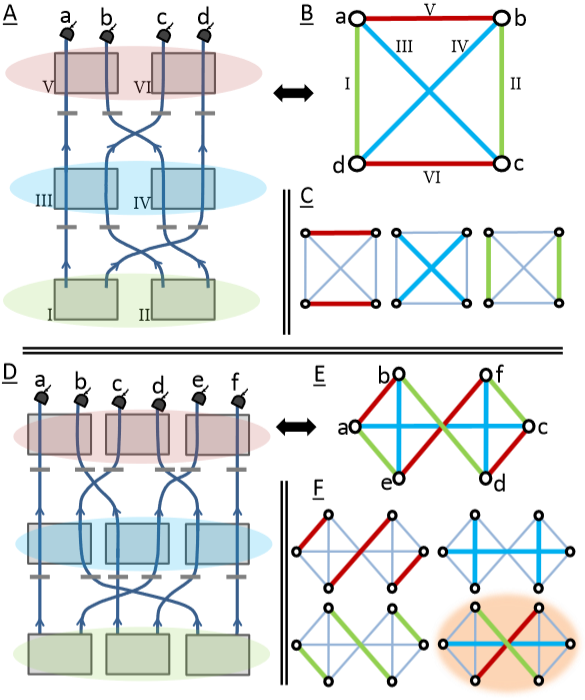
\includegraphics[scale=0.7]{figures/problem_presentation/motivations/krenn_graph}
    \caption{This figure was taken from Mario Krenn's paper of 2017 \cite{Krenn_2017}.
        It represents two examples of experiments to create entangled states using photonic technologies.
        On one hand, the experiment described in $A$ corresponds to the graph $B$ that is monochromatic as shown in $C$.
        Therefore, it allows to create a GHZ-state of dimension 3 involving four particles $\ket{\psi} = GHZ_{4, 3} = \frac{1}{\sqrt{3}} (\ket{0000} + \ket{1111} + \ket{2222})$.
        On the other hand, the experiment described in $D$ is represented by the graph in $E$, which is non-monochromatic as shown in $F$.
        Therefore, the state it creates is not a GHZ-state.
        $\ket{\psi'} = \frac{1}{2} (\ket{000000} + \ket{111111} + \ket{222222} + \ket{121200})$.}
    \label{fig:krenn_experiment}
\end{figure}

At last, please note that the study of GHZ-states is considered as a fundamental question in quantum physics.
For instance, Alain Aspect, John F. Clauser and Anton Zeilinger received in 2022 a Nobel Prize for their experiments on quantum entanglement, and their work was closely related to the topic~\cite{nobelprizeNobelPrize}.
Finding new ways to experimentally create such states would open new intriguing gates in the fields of quantum computing~\cite{gu2020compact} and cryptography~\cite{pivoluska2018layered}.\\

\chapter{State of the art}
\label{ch:state-of-the-art}

During the last few years, the problem was studied by a few researchers around the world.\cite{Krenn_2017,bogdanov,chandran,chandran2023graphtheoretic}
While none of them could find any constant upper bound on the weighted matching index of perfectly monochromatic graphs (defined in definitions~\ref{def:weighted_matching_index} and~\ref{def:perfectly_monochromatic_graph}), some special cases of the conjecture were proven to be true.
Furthermore, non-constant bounds could also be found in more general cases of experiment graphs.
This section aims to present these results.
But before getting started, it could be interesting to introduce some useful definitions and tools that will be used a lot during the different seen proofs.

\begin{definition}[(Non-)redundant experiment graph]
    \label{def:redundant-experiment-graph}
    In the context of this master thesis, an experiment graph $G_k^w$ as defined in definition~\ref{def:experiment_graph} is said to be \textit{non-redundant} if it satisfies all the following properties.

    \begin{itemize}
        \item $\forall e \in E(G), w(e) \neq 0$
        \item $\forall e \in E(G), \exists$ A perfect matching $M$ such that $e \in M$
        \item $\forall (v_1, v_2) \in (V(G))^2, v_1 \neq v_2,$ and $\forall$ colour pair $(r, g)$, $\exists$ at most one unique edge $e$ between $v_1$ and $v_2$ such that $k(e, v_1) = r$ and $k(e, v_2) = g$, using notations introduced in definition~\ref{def:mixed_edge_coloured_graph}.
    \end{itemize}

    Otherwise, it is said to be \textit{redundant}.
\end{definition}


\begin{definition}[Non-redundant induced graph]
    \label{def:non_redundant_induced_subgraph}
    Let $G_k^w$ be a redundant experiment graph.
    Then its \textit{non-redundant-induced graph} is the graph built by doing successively the following operations.

    \begin{itemize}
        \item $\forall e \in E(G)$ such that $w(e) = 0$, delete $e$.
        \item $\forall e \in E(G)$ that does not belong to any perfect matching $M$ of $G_k^w$, delete $e$.
        \item $\forall (v_1, v_2) \in (V(G))^2, v_1 \neq v_2$ And $\forall$ colour pair $(r, g)$, if there are multiple edges $e_1, e_2, \dots, e_m$ such that
        
        \begin{center}
            $\forall i \in \{1, \dots, m\}$, $k(e_i, v_1) = r$ and $k(e_i, v_2) = g$
        \end{center}
        Then, replace them by one single edge $e = (v_1, v_2)$ that has the following properties.
        
        \begin{center}
            $k(e, v_1) = r$ And $k(e, v_2) = g$ \\
            $w(e) = \sum\limits_{i = 1}^m w(e_i)$
        \end{center}
        
    \end{itemize}
    
\end{definition}

This definition and denomination is entirely motivated by the following observation.

\begin{observation}[Non-redundancy is enough]
    \label{obs:non_redundancy_enough}
    Let $G_k^w$ be a redundant experiment graph, and let ${G'}_{k'}^{w'}$ be its non-redundant induced graph. Then $\Tilde{c}(G, k, w) = \Tilde{c}(G', k', w')$.
\end{observation}

\begin{proof}
    To prove this last observation, the procedure will be to show that each of the transformations that was applied on $G_k^w$ did not change its weighted matching index.

    \begin{enumerate}
        \item \textbf{Transformation 1 :} $\forall e \in E(G)$ such that $w(e) = 0$, delete $e$. \\
            Let $e = (v_1, v_2)$ be a zero-weighted edge of $G_k^w$. At most, $e$ can contribute to the weights of all the feasible vertex colourings $\kappa$ such that $\kappa(v_1) = k(e, v_1)$ and $\kappa(v_2) = k(e, v_2)$. But since $w(e) = 0$, then all the perfect matchings $M$ such that $e \in M$ have a weight $w(M) = 0$. Therefore, $e$'s contribution to $\kappa$ is null, and removing it doesn't change anything to the feasibility of $\kappa$.

        \item \textbf{Transformation 2 :} $\forall e \in E(G)$ that do not belong to any perfect matching $M$ of $G_k^w$, delete $e$. \\
            Since $e$ does not belong to any perfect matching $M$, its weight can not contribute to any feasible vertex colouring $\kappa$. Removing it has therefore no impact.

        \item \textbf{Transformation 3 :} $\forall (v_1, v_2) \in (V(G))^2, v_1 \neq v_2$ and $\forall$ colour pair $(r, g)$, if there are multiple edges $e_1, e_2, \dots, e_m$ such that
        \begin{center}
            $\forall i \in \{1, \dots, m\}$, $k(e_i, v_1) = r$ and $k(e_i, v_2) = g$
        \end{center}
        Then, replace them by one single edge $e = (v_1, v_2)$ that has the following properties.
        \begin{center}
            $k(e, v_1) = r$ And $k(e, v_2) = g$ \\
            $w(e) = \sum\limits_{i = 1}^m w(e_i)$
        \end{center}

            Indeed, let $\kappa$ be a feasible vertex colouring such that $\kappa(v_1) = r$ and $\kappa(v_2) = g$. We need to introduce some new notations for this specific part of the proof, which are inspired of the notations we previously defined in definition \ref{def:induced_vertex_colouring} of an induced vertex colouring.

            \begin{itemize}
                \item $\mathcal{M}_\kappa$ Is the set of all perfect matching $M$ of $G$ that induce a vertex colouring $\kappa$ on $G$.
                \item $\mathcal{M}_\kappa^{e_i}$ Is the set of perfect matchings $M$ of $G$ that induce a vertex colouring $\kappa$ on $G$ such that $e_i \in M$.
                \item $\mathcal{M}_\kappa^{*}$ Is the set of perfect matchings $M$ of $G$ that have no edges from $\{e_1, \dots, e_m\}$.
                \item $\mathcal{M'}_\kappa$ Is the set of all perfect matching of $G'$ that induce a vertex colouring $\kappa$ on $G'$.
                \item $\mathcal{M'}_\kappa^{e}$ Is the set of perfect matchings of $G'$ that induce a vertex colouring $\kappa$ on $G'$ such that $e_i \in M$.
                \item $\mathcal{M'}_\kappa^{*} = \mathcal{M}_\kappa^{*}$ Is the set of perfect matchings $M$ of $G'$ that have do not contain $e$.
            \end{itemize}

            Using these new notations, and by the definition \ref{def:vertex_colouring_weight} of the weight of a vertex colouring, 

            \begin{center}
                $\begin{array}{r c l}
                    w(\kappa) & = & \sum\limits_{M \in \mathcal{M}_\kappa} w(M)  \\
                              & = & \sum\limits_{i = 1}^m \sum\limits_{M \in \mathcal{M}_\kappa^{e_i}} w(M) + \sum\limits_{M \in \mathcal{M}_\kappa^{*}} w(M) \\
                              & = & \sum\limits_{i = 1}^m w(e^i) \sum\limits_{M \in \mathcal{M}_\kappa^{e_i}} w(M \backslash e^i) + \sum\limits_{M \in \mathcal{M}_\kappa^{*}} w(M) \\
                              & = & w(e) \sum\limits_{M \in \mathcal{M'}_\kappa^{e}} w(M \backslash e) + \sum\limits_{M \in \mathcal{M'}_\kappa^{*}} w(M) \\
                              & = & \sum\limits_{M \in \mathcal{M'}_\kappa} w(M)
                \end{array}$
            \end{center}

            This result proves the transformation 3 did not have any influence on the weight of all induced vertex colourings.
    \end{enumerate}
\end{proof}

This last observation is convenient since it allows researchers to focus on non-redundant experiment graphs to prove bounds on their matching index, and these bounds are still valid in redundant experiment graphs without any loss of generality. An example of such transformation is shown in figure \ref{fig:non_redundant_induced_graph}.

\begin{figure}[H]
    \ctikzfig{figures/state_of_the_art/non_redundant_induced_graph}
    \caption{In this figure, $G_k^w$ is an experiment graph and ${G'}_{k'}^{w'}$ is its non-redundant induced graph. In this particular case, it consisted in doing the following operations. First of all, the $0$-weighted edge between $v_3$ and $v_6$ is removed. Secondly, the edge $\{v_1, v_3\}$ is also deleted because it does not belong to any perfect matching (indeed, including it in a perfect matching $M$ would prevent $M$ to cover $v_2$). Lastly, the two edges between $v_4$ and $v_6$ are combined in one single edge, since they have the same colour at each endpoint. The reader can verify that the resulting graph ${G'}_{k'}^{w'}$ has a weighted matching index $\Tilde{c}(G', k', w') = 2$. Therefore, $\Tilde{c}(G, k, w) = 2$ by observation \ref{obs:non_redundancy_enough}.}
    \label{fig:non_redundant_induced_graph}
\end{figure}


\section{Special cases that were already proven}

\subsection{Restrictions on the weights}

\begin{lemma}[Real, positive weights]
    \label{lem:real_pos_weights}
    Let $G_k^w$ be a perfectly monochromatic graph which has only positive, real weights. If $G$ is isomorphic to $K_4$, then $\Tilde{c}(G, k, w) \leq 3$. Otherwise, $\Tilde{c}(G, k, w) \leq 2$.
\end{lemma}

\begin{proof}
    This is a direct result from Bogdanov's proof, described in theorem \ref{thm:bogdanov}. \cite{bogdanov}. Because all the weights of $G_k^w$ are real, positive numbers, it means that the weight of any perfect matching is positive. Therefore, the weight of any feasible vertex colouring is positive by definition \ref{def:vertex_colouring_weight}. But all the non-monochromatic feasible vertex colourings in a perfectly monochromatic graph should have a weight of 0 by definition \ref{def:monochromatic_graph}. It follows that $G_k^w$ has no non-monochromatic perfect matching. Then $\Tilde{c}(G, k, w) = c(G, k)$.
\end{proof}


\subsection{Restrictions on the matching index}

In 2022, Gajjala and Chandran analysed the Krenn's conjecture by separating the graphs in different subclasses according to their matching index (see definition \ref{def:matching_index}). Here are their results.

\begin{lemma}[Graphs with a matching index of 0]
    \label{lem:if_c_is_0}
    If $G$ is a a graph with a matching index of 0, then the Krenn's conjecture is true for $G$ and $\Tilde{c}(G) = c(G) = 0$.
\end{lemma}

\begin{proof}
    Let $G$ be a a graph with a matching index of 0. Then, $G$ has no perfect matchings (otherwise it would be feasible to colour all the edges of $G$ in the same colour and find a monochromatic perfect matching, which contradicts the fact that $c(G) = 0$ by definition \ref{def:matching_index} of a matching index). Because it has no perfect matchings, there is no mixed-edge colouring $k$ and weight attribution $w$ such that $G_k^w$ has a feasible monochromatic vertex colouring. It follows that $\Tilde{c}(G) = 0$.
\end{proof}

\begin{lemma}[Graphs with a matching index of 2]
    \label{lem:if_c_is_2}
    If $G$ is a a graph with a matching index of 2, then the Krenn's conjecture is true for $G$ and $\Tilde{c}(G) = c(G) = 2$.
\end{lemma}

This last lemma is proved by Chandran and Gajjala in \cite{chandran}. The proof is not trivial and uses some very interesting observations about the structure of a perfectly monochromatic graph with $\Tilde{c}(G) = 2$. The reader is highly encouraged to have a look at it in the original paper in order to believe this claim. Nevertheless, the proof will not be discussed here since it would be a bit redundant. Thanks to their proof, Chandran and Gajjala could pose the following theorem, which is a summary of the 2 last lemmas \ref{lem:if_c_is_0} and \ref{lem:if_c_is_2}.

\begin{theorem}[Chandran - Gajjala's theorem]
    \label{thm:c_not_1}
    Let $G$ be a perfectly monochromatic graph. If $c(G) \neq 1$, then the Krenn's conjecture is true and $\Tilde{c}(G) = c(G)$.
\end{theorem}

Having that last theorem, it would be a natural question to ask ourselves if, for any graph $G$, $c(G) = \Tilde{c}(G)$. Unfortunately, it is not the case, since a counter-example was found by Chandran and Gajjala. \cite{chandran}

\begin{observation}
    \label{obs:c_not_c_tilde}
    There exists a graph $G$ that satisfies $c(G) = 1$ and $\Tilde{c}(G) = 2$. This counter example is shown in figure \ref{fig:proof_c_not_c_tilde}.
\end{observation}

\begin{figure}[H]
    \ctikzfig{figures/state_of_the_art/special_cases/c_not_c_tilde}
    % TODO : there's an error here and in the other similar figure
    \caption{Example of graph $G$ that has a matching index of $1$ and a weighted matching index of $2$. On this figure, the edge-colouring $k$ is an example of edge colouring that gives $c(G, k) = 1$. Furthermore, the mixed-edge colouring $k'$ and the weight attribution $w$ are examples of mixed-edge colourings and weights attributions that results in $\Tilde{c}(G, k', w) = 2$. Another example of mixed-edge colouring and weight attribution that gives the same matching index on $G$ is available in figure \ref{fig:perfectly_mono}. It has still to be shown that it is impossible to find other edge-colourings / weight attributions that would lead to bigger (weighted) matching indexes. This proof is not presented here, but is available in Chandran and Gajjala's original paper. \cite{chandran}}
    \label{fig:proof_c_not_c_tilde}
\end{figure}


\section{Known non-constant bounds on the weighted matching index}

Despite the failure to find any constant bound on the weighted matching index of experiment graphs up to now, some interesting non-constant bounds were nevertheless found. Chandran and Gajjala discovered in \cite{chandran} two interesting bounds in terms of minimum degree and edge connectivity that I considered to be relevant to rewrite here. The 2 following theorems are due to them.

\begin{lemma}[Upper bound in terms of minimum degree]
    \label{lem:bound_min_degree}
    Let $G$ be a graph, and $\delta(G)$ be its minimum degree as defined in definition \ref{def:degree}. Then $\Tilde{c}(G) \leq \delta(G)$.
\end{lemma}

\begin{proof}
    Let $G_k^w$ be a perfectly monochromatic graph such that $\Tilde{c}(G, k, w) = \Tilde{c}(G)$. It is known by definition \ref{def:weighted_matching_index} of the weighted matching index that $G_k^w$ has at least one monochromatic perfect matching for $\Tilde{c}(G)$ different colour classes. In the context of this proof, these perfect matchings are denoted $M_1, M_2, \dots, M_{\Tilde{c}(G)}$. Because these perfect matchings are of different colours, they can not share any edge.\\
    
    Let $v \in V(G)$ be a vertex of minimum degree $d(v) = \delta(G)$. This vertex must be covered by $M_1, M_2, \dots, M_{\Tilde{c}(G)}$. $M_1$ Covers it through an edge $e_1$, $M_2$ through an edge $e_2$, $\dots$, $M_{\Tilde{c}(G)}$ through an edge $e_{\Tilde{c}(G)}$ (as shown in figure \ref{fig:proof_min_degree}). Then $v$ has at least $\Tilde{c}(G)$ outgoing edges, and $d(v) = \delta(G) \geq \Tilde{c}(G)$.
\end{proof}

\begin{figure}[H]
    \ctikzfig{figures/state_of_the_art/known_bounds/proof_min_degree}
    \caption{Visualisation of the proof that $\Tilde{c}(G) \leq \delta(G)$ for every perfectly monochromatic graph $G$.}
    \label{fig:proof_min_degree}
\end{figure}

\begin{theorem}[Upper bound in terms of edge connectivity]
    \label{thm:bound_edge_connectivity}
    Let $G$ be a graph, and $\lambda(G)$ be its edge connectivity as defined in definition \ref{def:edge_connectivity}. Then $\Tilde{c}(G) \leq \lambda(G).$
\end{theorem}

The proof of this last theorem is not trivial and uses some concepts that need to be properly defined here. It was first described by Chandran and Gajjala in \cite{chandran}, and we are using the same concepts than them here.

\begin{definition}[Redundant edge]
    \label{def:redundant_edge}
    An edge $e$ from a graph $G$ is said to be \textit{redundant} if it does not belong to any perfect matching of $G$.
\end{definition}

\begin{definition}[Redundant colour class]
    \label{def:redundant_colour_class}
    A colour class $r$ from an edge colouring $k$ of a graph $G$ is said to be \textit{redundant} if there are no monochromatic perfect matching of colour $r$ in $G_k$.
\end{definition}

\begin{definition}[Redundant mixed-colour class]
    \label{def:redundant_mixed_colour_class}
    A mixed-colour class $(r, b)$ from an edge-colouring $k$ of a graph $G$ is said to be \textit{redundant} if at least one of the 2 following conditions is true.
    \begin{center}
        $\left\{
        \begin{array}{l}
            r \mbox{ is a redundant colour class} \\
            b \mbox{ is a redundant colour class}
        \end{array}
        \right.$
    \end{center}
\end{definition}

\begin{proof}[Proof of Theorem \ref{thm:bound_edge_connectivity}]
    This theorem is proven by contradiction. Using the notations introduced in definitions \ref{def:weighted_matching_index} and \ref{def:edge_connectivity}, let assume there exists a graph $G''$ such that $\Tilde{c}(G'') \geq \lambda(G'') + 1$. By removing all the redundant edges (defined in definition \ref{def:redundant_edge}) of $G''$, it results in a graph $G'$ with $\Tilde{c}(G'') = \Tilde{c}(G')$. This manipulation preserves the weighted matching index of the graph.
    
    \begin{center}
        $\Tilde{c}(G') \geq \lambda(G'') + 1$
    \end{center}
    
    Therefore, there exists a mixed-edge colouring $k'$ and a weight attribution $w'$ such that
    
    \begin{center}
        $\Tilde{c}(G') = \Tilde{c}(G', k', w') \geq \lambda(G'') + 1$
    \end{center}
    
    From ${G'_{k'}}^{w'}$, let apply a new transformation that removes all edges that belong to a redundant colour class and all edges that belong to a redundant mixed-colour class (defined in definitions \ref{def:redundant_colour_class} and \ref{def:redundant_mixed_colour_class}), obtaining $G_k^w$. It is easy to see that, if ${G'_{k'}}^{w'}$ was perfectly monochromatic, $G_k^w$ is still perfectly monochromatic. Indeed, by removing all the edges from a redundant colour class, no monochromatic perfect matching is removed (since the colour class was redundant) and, if there were (non-monochromatic) perfect matchings containing edges of that colour class, they are all destroyed, so there is no induced vertex colouring of $G$ anymore that has vertices of the removed colour class - then it's not needed anymore to worry about the weight of such vertex colourings. \\
    
    $\Tilde{c}(G)$ Did not decrease, because no non-redundant colour class was removed from ${G'_{k'}}^{w'}$, and did not increase, since removing edges can not create new perfect matchings. So again :
    
    \begin{center}
        $\Tilde{c}(G) = \Tilde{c}(G') = \Tilde{c}(G'')$
    \end{center}
    
    We also notice that the edge-connectivity of a graph can not increase when we remove edges. Therefore
    
    \begin{center}
        $\begin{array}{l c l}
            \Tilde{c}(G) & \geq & \lambda(G'') + 1 \\
                         & \geq & \lambda(G') + 1 \\
                         & \geq & \lambda(G) + 1
        \end{array}$
    \end{center}
    
    By definition \ref{def:edge_connectivity} of the edge-connectivity of a graph, $G$ can be cut in 2 disconnected components $S$ and $S'$ by removing $\lambda(G)$ edges. Note that, if $G$ has perfect matchings, $|V(G)|$ is an even number and therefore $|S|$ and $|S'|$ are of the same parity.
    
    \begin{enumerate}
        \item 
            \textbf{If $|S|$ and $|S'|$ are odd} then, for all monochromatic perfect matching $M$, $M$ contains at least one crossing edge, i.e. an edge with one endpoint in $S$ and the other endpoint in $S'$ (see figure \ref{fig:proof_lambda_odd}).
            
            \begin{figure}[H]
                \ctikzfig{figures/state_of_the_art/known_bounds/proof_lambda_odd}
                \caption{Existence of a crossing edge between $S$ and $S'$ in a perfect matching $M$ of $G$ if $|S|$ and $|S'|$ are odd.}
                \label{fig:proof_lambda_odd}
            \end{figure}
            
            Let $E(S, S')$ be the set of crossing edges from $S$ to $S'$. The maximum number of different colour classes that can be found on $E(S, S')$ is $\lambda(G)$ (otherwise more edges wold be needed). The conclusion is that the monochromatic perfect matchings of $G_k^w$ can be of a most $\lambda(G)$ different colours. Hence,
            
            \begin{center}
                $\Tilde{c}(G'') = \Tilde{c}(G) \leq \lambda(G) \leq \lambda(G'')$
            \end{center}
            
            This forms a contradiction with the statement that $\Tilde{c}(G'') \geq \lambda(G'') + 1$.
            
        \item
            \textbf{If $|S|$ and $|S'|$ are even} then let's separate all the colour classes of $G_k^w$ in
            
            \begin{center}
                $\left\{ \begin{array}{l c l c l}
                    [r]             & = & \{1, 2, \dots, r\}              & = & \mbox{all the colours such that none of the monochromatic} \\
                                    &   &                                 &   & \mbox{perfect matchings of these colours intersects } E(S, S') \\ 
                    {[r + 1, r + r']} & = & \{r + 1, r + 2, \dots, r + r'\} & = & \mbox{all the colours such that there exists a monochromatic} \\
                                    &   &                                 &   & \mbox{perfect matching of this colour intersecting } E(S, S')
                \end{array} \right.$
            \end{center}
            
            Clearly, $\Tilde{c}(G'') = \Tilde{c}(G) = r + r'$. For all colours $i \in [r + 1, r + r']$, there exists a monochromatic perfect matching $M$ which intersects $E(S, S')$. And since $|S|$ and $|S'|$ are even, $M$ contains at least 2 edges from $E(S, S')$, as shown in figure \ref{fig:proof_lambda_even}.
            
            \begin{figure}[H]
                \ctikzfig{figures/state_of_the_art/known_bounds/proof_lambda_even}
                \caption{Existence of $2$ crossing edges in a crossing perfect matching $M$ of $G$ if $|S|$ and $|S'|$ are even numbers.}
                \label{fig:proof_lambda_even}
            \end{figure}
            
            Then there exist at least 2 edges of colour $i$ in $E(S, S')$ for all $i \in [r + 1, r + r']$. It follows that $\lambda(G'') \geq \lambda(G) \geq 2 \cdot r'$.
            
            \begin{enumerate}
                \item 
                    \textbf{If $r \leq 1$ and $r' \geq 1$}, then 
                    
                    \begin{center}
                        $\begin{array}{l c l}
                            \Tilde{c}(G'')  & =    & r + r' \\
                                            & \leq & 2 \cdot r' \\
                                            & \leq & \lambda(G'')
                        \end{array}$
                    \end{center}
                    
                \item 
                    \textbf{If $r \leq 1$ and $r' = 0$}, then it is trivial because $G$ is connected.
                    
                    \begin{center}
                        $\begin{array}{lcl}
                            \lambda(G'')  & \geq & 1 \\
                                          & \geq & r + r' \\
                                          & =    & \Tilde{c}(G'')
                        \end{array}$
                    \end{center}
                    
                \item
                    \textbf{Else, $r \geq 2$}. Then one can pick 2 colours from $[r]$ (let say $1$ and $2$).
                    
                    \begin{claim}
                        There should be at least 2 mixed edges of colour $(1, 2)$ in $E(S, S')$.
                    \end{claim}
                    
                    \begin{proof}[Proof of the claim]
                        By contradiction, suppose not. Let's consider 2 monochromatic perfect matchings $M_1$ and $M_2$ of colour $1$ and $2$ that induce the monochromatic vertex colourings $1_{V(G)}$ and $2_{V(G)}$ respectively. $M_1$ And $M_2$ do not have any edge in $E(S, S')$. In general in the context of this proof, $i_A$ will denote the monochromatic vertex colouring of colour $i$ of the vertices in $A$. Because $G_k^w$ is perfectly monochromatic, the weights of $1_{V(G)}$ and $2_{V(G)}$ must be $1$. Since $1, 2 \in [r]$, there are no normal edges of colour $1$ nor $2$ in $E(S, S')$. Then we have the following relations, where $w(i_A)$ denotes the weight of the the monochromatic vertex colouring of colour $i$ on the subgraph $A$.
                        
                        \begin{center}
                            $\begin{array}{l c l c l}
                                w(1_{V(G)}) & = & w(1_S) \cdot w(1_{S'}) & = & 1 \\
                                w(2_{V(G)}) & = & w(2_S) \cdot w(2_{S'}) & = & 1
                            \end{array}$
                        \end{center}
                        
                        Therefore, $w(1_S)$, $w(1_{S'})$, $w(2_S)$, $w(2_{S'})$ must be non-zeros. \\

                        Now let's consider a non-monochromatic vertex colouring $\kappa$ in which $S$ is coloured $1$ and $S'$ is coloured $2$. $\kappa$ Is feasible because we can build a perfect matching by taking all the edges from $M_1$ on $S$ and all the edges from $M_2$ on $S'$. Because $G_k^w$ is perfectly monochromatic, $w(\kappa)$ is 0 by definition \ref{def:perfectly_monochromatic_graph}. Also, since $|S|$ and $|S'|$ are even, every perfect matching contains an even number of edges from $E(S, S')$. But by assumption, there is at most one crossing edge of colour $\{1, 2\}$ and no crossing edges of colour $1$ nor $2$. In conclusion, no perfect matching that induces $\kappa$ can contain an edge from $E(S, S')$. Then
                        
                        \begin{center}
                            $w(\kappa) = w(1_S) \cdot w(2_{S'}) = 0$
                        \end{center}
                        
                        But $w(1_S)$ and $w(2_{S'})$ are non-zeros, so this is impossible and creates a contradiction. This proves the claim.
                    \end{proof}

                    \textbf{We proved our claim.} Therefore, for a pair of colours $i, j \in [r]$, there should be at least 2 mixed edges of colour $\{i, j\}$ in $\{S, S'\}$.
                    
                    \begin{center}
                        Minimum number of edges in $E(S, S') = 2 {r \choose 2} + 2 \cdot r' \leq \lambda(G'')$
                    \end{center}
                    
                    Finally, it means that
                    
                    \begin{center}
                        $\begin{array}{lcl}
                            \Tilde{c}(G'') & =    & r + r' \\
                                           & \leq & 2 {r \choose 2} + 2 \cdot r' \\
                                           & \leq & \lambda(G'')
                        \end{array}$
                    \end{center}
                    
                    And this ends the proof.
            \end{enumerate}
    \end{enumerate}
\end{proof}

This proof was interesting to rewrite here since it uses some very interesting reasoning about the structure of perfectly monochromatic graphs and the definitions of their weights. Some similar reasoning is sometimes reused in this master thesis in order to prove my own new results. \\

Last but not least, Chandran and Gajjala showed more recently an upper bound on the weighted matching index of graphs in term of their number of vertices. \cite{chandran2023graphtheoretic}

\begin{theorem}[Upper bound in terms of number of vertices]
    \label{thm:bound_num_vertices}
    Let $G_k^w$ be an experiment graph that has $n$ vertices. Then
    \begin{center}
        $\Tilde{c}(G, k, w) \frac{n}{\sqrt{2}}$
    \end{center}
\end{theorem}

The proof of theorem \ref{thm:bound_num_vertices} is detailed in Chandran and Gajjala's publication \cite{chandran2023graphtheoretic}.


\section{Computational approach}
\chapter{New theoretical contributions}
\label{ch:new-contributions}

There are two intuitive ways to tackle the problem of the Krenn's conjecture.
The first way, done in this chapter, is to use a theoretical approach to find interesting properties about perfectly monochromatic graphs.
In this approach, I prove the Krenn's conjecture in a very restrained subcase in subsection~\ref{subsec:one_negative_edge}.
Then, I show how to relax the constraints of this analysed subcase in the subsection~\ref{subsec:2-pos-classes}.
Also, I present two different ways of thinking to the problems by showing an equivalency between two cases in the subsection~\ref{sec:problem-reduction}.\\

The second approach is a computational approach, and is presented in chapter~\ref{ch:computational-approach}.
The goal of this second approach will be to generate a big number of random perfectly monochromatic experiment graphs, and extract conclusions from the data.
To do so, I will present a new tool I developed, called EGPI, that aims to perform such experiments.


\section{Problem reduction}
\label{sec:problem-reduction}

Let $\beta \in \mathbb{N}_0$ be a strictly positive integer.
Having $\beta$, we can formulate the two following conjectures.

\begin{conjecture}[Weighted matching index bounded by $\beta$ if binary weights]
    \label{con:c-bounded-by-beta-binary}
    Let $\forall {G_\mu}^w$ be a perfectly monochromatic graphs such that $w: E(G) \rightarrow \{-1, 1\}$.
    Then, $\Tilde{c}(G, \mu, w) \leq \beta$.
\end{conjecture}

\begin{conjecture}[Weighted matching index bounded by $\beta$ if integer weights]
    \label{con:c-bounded-by-beta-integer}
    Let $\forall {G_\mu}^w$ be a perfectly monochromatic graphs such that $w: E(G) \rightarrow \mathbb{Z}$.
    Then, $\Tilde{c}(G, \mu, w) \leq \beta$.
\end{conjecture}

Since the conjecture~\ref{con:c-bounded-by-beta-binary} seems to be a particular case of the conjecture~\ref{con:c-bounded-by-beta-integer}, the conjecture~\ref{con:c-bounded-by-beta-binary} seems to be easier to prove.
However, the following lemma holds.

\begin{lemma}[Conjectures \ref{con:c-bounded-by-beta-binary} and \ref{con:c-bounded-by-beta-integer} are equivalent]
    \label{lem:pm_graphs_with_integer_weights}
    Let $\beta \in \mathbb{N}_0$ be a strictly positive integer.
    The conjecture~\ref{con:c-bounded-by-beta-binary} is true for $\beta$ if and only if the conjecture~\ref{con:c-bounded-by-beta-integer} is true for $\beta$.
    In other words, the two conjectures are equivalent.
\end{lemma}

\begin{proof}[Proof of Lemma \ref{lem:pm_graphs_with_integer_weights}]
    Let $G_\mu^w$ be a perfectly monochromatic graph that has only edge weights included in $\mathbb{Z}$.
    We will show that we can build a perfectly monochromatic graph that has only weights included in $\{-1, 1\}$ and that has the same weighted matching index than $G_\mu^w$. \\

    First, we choose an edge in $G_\mu^w$ that has a weight different from $1$ or $-1$ (if such an edge doe not exist, we are done).
    We replace this edge by $|w(e)|$ parallel edges of the same colour, and that have all a weight of $\frac{w(e)}{|w(e)|}$ (1 if $w(e) > 0$, -1 if $w(e) < 0$).
    We say that each of these new edges is \textit{derived} from $e$.
    Remember this can be done because experiment graphs allow multi-edges by definition~\ref{def:experiment_graph}.
    This creates a new graph ${G'_{\mu'}}^{w'}$.
    That process is illustrated in figure~\ref{fig:demo_integers}.\\

    \begin{figure}[H]
        \ctikzfig{figures/new_results/problem_reduction/demo_integers}
        \caption{Illustration of the transformation from an experiment graph with integer weights to an experiment graph with weights included in $\{-1, 1\}$.}
        \label{fig:demo_integers}
    \end{figure}

    Let $\kappa$ be a feasible vertex colouring of $G_\mu^w$.
    To compute the weight of $\kappa$ in $G_\mu^w$, we will denote by
    \begin{center}
        $\left\{
            \begin{array}{ll}
                M_{\kappa}          & \mbox{the set of perfect matchings of } G_\mu^w \mbox{ that induce the vertex colouring } \kappa \\
                M_{\kappa}^e        & \mbox{the set of perfect matchings of } G_\mu^w \mbox{ that induce the vertex colouring } \kappa \mbox{ and contain } e \\
                M_{\kappa}^{\neg e} & \mbox{the set of perfect matchings of } G_\mu^w \mbox{ that induce the vertex colouring } \kappa \mbox{ and do not contain } e
            \end{array}
        \right.$
    \end{center}

    The weight of $\kappa$ in $G_\mu^w$ is

    \begin{center}
        $\begin{array}{lclcl}
            w(\kappa \mbox{ in } G_\mu^w)
                & = & \sum\limits_{M \in M_{\kappa}} w(M) \\
                & = & \sum\limits_{M \in M_{\kappa}^{\neg e}} w(M) & + & \sum\limits_{M \in M_{\kappa}^{e}} w(M)
        \end{array}$
    \end{center}

    The next step, which is the heart of the proof, consists of computing the weight of the vertex colouring $\kappa$ in ${G'_{\mu'}}^{w'}$.
    We will denote by

    \begin{center}
        $\left\{
            \begin{array}{ll}
                M'_{\kappa}            & \mbox{the set of perfect matchings of } {G'_{\mu'}}^{w'} \mbox{ that induce the vertex colouring } \kappa \\
                {M'_{\kappa}}^e        & \mbox{the set of perfect matchings of } {G'_{\mu'}}^{w'} \mbox{ that induce the vertex colouring } \kappa \\
                                   & \mbox{and contain an edge that was derived from } e \\
                {M'_{\kappa}}^{\neg e} & \mbox{the set of perfect matchings of } {G'_{\mu'}}^{w'} \mbox{ that induce the vertex colouring } \kappa \\
                                   & \mbox{and does not contain an edge that was derived from } e
            \end{array}
        \right.$
    \end{center}

    In addition to these concepts, for every perfect matching $M \in M_{\kappa}^e$, let $\mathcal{M}'(M)$ be the set of corresponding perfect matchings $M'$ in ${M'_{\kappa}}^e$.
    In other words, $\mathcal{M}'(M)$ denotes the perfect matchings that are the same as $M$ on every edge except $e$, and that contain one of the edges that were added when $e$ was removed.
    It follows that, for every $M \in M_{\kappa}^e$, $|\mathcal{M}'(M)| = w(e)$.
    Also, given $M \in M_{\kappa}^e$, for each perfect matching $M' \in \mathcal{M}'(M)$, $w(M') = \frac{w(M)}{|w(e)|}$.
    Finally, we notice the following relations between the different sets we defined :

    \begin{center}
        $\left\{
            \begin{array}{lcl}
                {M'_{\kappa}}^{\neg e} & = & M_{\kappa}^{\neg e} \\
                {M'_{\kappa}}^e        & = & \bigcup\limits_{M \in M_{\kappa}^e} \mathcal{M}'(M)
            \end{array}
        \right.$
    \end{center}

    Having all these observations in mind, we can now compute the weight of $\kappa$ in ${G'_{\mu'}}^{w'}$.

    \begin{center}
        $\begin{array}{lclcl}
            w(\kappa \mbox{ in } {G'_{\mu'}}^{w'})
                & = & \sum\limits_{M' \in M'_{\kappa}} w(M') \\
                & = & \sum\limits_{M' \in {M'_{\kappa}}^{\neg e}} w(M') & + & \sum\limits_{M' \in {M'_{\kappa}}^{e}} w(M') \\
                & = & \sum\limits_{M \in {M_{\kappa}}^{\neg e}} w(M)    & + & \sum\limits_{M \in M_{\kappa}^e} \left( \sum\limits_{M' \in \mathcal{M}'(M)} w(M') \right) \\
                & = & \sum\limits_{M \in {M_{\kappa}}^{\neg e}} w(M)    & + & \sum\limits_{M \in M_{\kappa}^e} \left( \sum\limits_{M' \in \mathcal{M}'(M)} \frac{w(M)}{|w(e)|} \right) \\
                & = & \sum\limits_{M \in {M_{\kappa}}^{\neg e}} w(M)    & + & \sum\limits_{M \in M_{\kappa}^e} \left( |w(e)| \frac{w(M)}{|w(e)|} \right) \\
                & = & \sum\limits_{M \in {M_{\kappa}}^{\neg e}} w(M)    & + & \sum\limits_{M \in M_{\kappa}^e} w(M) \\
                & = & w(\kappa \mbox{ in } G_\mu^w)
        \end{array}$
    \end{center}

    So, since the weight of each feasible vertex colouring in $G_\mu^w$ remains unchanged in ${G'_{\mu'}}^{w'}$, the monochromatic feasible vertex colourings have still a weight of 1, and the non-monochromatic feasible vertex colourings have still a weight of 0.
    So, ${G'_{\mu'}}^{w'}$ is still perfectly monochromatic and $\Tilde{c}(G', \mu', w') = \Tilde{c}(G, \mu, w)$.
    Now, we can rename $G'$ as $G$ and repeat the whole procedure while $G_\mu^w$ has still edges with a weight different from $\{-1, 1\}$.
    The resulting graph has only edges that have signed unitary weights and has the same weighted chromatic index as the initial graph.
    So if any upper bound can be found on the weighted matching index of the final graph with signed unitary weights, it will still be valid for the weighted matching index of the initial one, with integer weights.
\end{proof}

The implication of Lemma~\ref{lem:pm_graphs_with_integer_weights} is that there are actually two ways to reason about the Krenn's conjecture when we are interested in integer weights.
The first way is to consider only non-redundant graphs (as defined in definition~\ref{def:redundant-experiment-graph}) and to try to find a bound on their weighted matching index.
And the second way is to consider redundant graphs in which each edge has a weight included in $\{-1, 1\}$.
Every result discovered in the second approach can be translated to the first approach, and vice versa.


\section{Constraints' relaxation}
\label{sec:constraints-relaxation}

As it was explained in the introduction, a simplified version of the conjecture was already proven thanks to Bogdanov.\cite{bogdanov}
This version, presented in Lemma~\ref{lem:real_pos_weights}, is only valid when all the weights of a perfectly monochromatic graph $G_\mu^w$ are positive.  % TODO: check if we can have bicoloured edges
In this section, our main goal will be to relax these constraints.

\subsection{Allowing one negative edge}
\label{subsec:one_negative_edge}

Since the conjecture is proven to be true when all the weights are positive, it is natural to ask ourselves how the proof would be affected if this constraint is relaxed.
The most simple case is the one where one edge is allowed to have a negative weight.
In this section, I show that the Krenn's conjecture is true for simple graphs in the absence of bicoloured edges and when maximum one edge has a negative weight.
Let's begin by proving the two following claims.

\begin{claim}[Existence of a Hamiltonian cycle]
    \label{clm:2_positive_classes_ham_cycle}
    Let $G_\eta^w$ be a perfectly monochromatic graph that respects the following properties.
    \begin{itemize}
        \item $G$ is a simple graph, referring to definition~\ref{def:simple_graph}.
        \item $\eta$ is a pure edge colouring, referring to definition~\ref{def:edge-coloured-graph}.
        \item $G_\eta^w$ has a weighted matching index $\Tilde{c}(G, \eta, w) \geq 3$.
        \item $\exists$ two colours $r, g \in \left(\eta(E(G))\right)^2, r \neq g$, such that all the edges coloured $r$ or $g$ in $G_\eta^w$ have a real, positive weight.
    \end{itemize}

    Let $M_r$ and $M_g$ be $2$ monochromatic perfect matchings of $G_\eta^w$ coloured $r$ and $g$ respectively.
    Then, the union of $M_r$ and $M_g$ forms a Hamiltonian cycle of even length.
\end{claim}

\begin{proof}[Proof of Claim \ref{clm:2_positive_classes_ham_cycle}]
    Since $M_r$ and $M_g$ are disjoint, they form a disjoint union $\mathcal{C}$ of cycles of even length.
    If $\left| \mathcal{C} \right| \geq 2$, we will denote by $C_i$ the $i^{th}$ cycle.
    Then, we can build the following non-monochromatic perfect matching :
    \begin{center}
        $N = (C_1 \cap M_r) \cup \left(\bigcup\limits_{i=2}^{\left| \mathcal{C} \right|} C_i \cap M_g\right)$
    \end{center}

    The construction of $N$ is highlighted in figure~\ref{fig:demo_unique_neg_ham}.

    \begin{figure}[H]
        \ctikzfig{figures/new_results/2_pos_classes/2_pos_classes_ham_cycle}
        \caption{In this example, the non-monochromatic perfect matching $N$ (represented by thick edges) is constructed from a red perfect matching and a blue one. The induced vertex colouring is also visible.}
        \label{fig:demo_unique_neg_ham}
    \end{figure}

    Since $M_r$ and $M_g$ include no negatively weighted edge, $w(N) > 0$.
    But, by definition~\ref{def:perfectly_monochromatic_graph} of a perfectly monochromatic graph, and using the notations introduced in definitions~\ref{def:matching_weight} and~\ref{def:feasible_vertex_colouring},

    \begin{center}
        $w(\kappa(N)) = \sum\limits_{N_i \in \mathcal{M}_{\kappa(N)}} N_i = 0$
    \end{center}

    Therefore, we know that $\exists N' \in \mathcal{M}_{\kappa(N)}$ such that $w(N') < 0$.
    This is impossible, because the only way for $N'$ to have a negative weight is to include at least one negative edge.
    And negative edges don't exist in colours $r$ or $g$.       % TODO: check if there are still nor's left
    We can conclude that $\left| \mathcal{C} \right| = 1$, which means that the union of $M_r$ and $M_g$ forms a Hamiltonian cycle.
\end{proof}

\begin{claim}[Parity of crossing edges]
    \label{clm:2_positive_classes_parity_crossing_edge}
    Let $G_\eta^w$ be a perfectly monochromatic graph that respects the following properties.
    \begin{itemize}
        \item $G$ is a simple graph, referring to definition~\ref{def:simple_graph}.
        \item $\eta$ is a pure edge colouring, referring to definition~\ref{def:edge-coloured-graph}.
        \item $G_\eta^w$ has a weighted matching index $\Tilde{c}(G, \eta, w) \geq 3$.
        \item $\exists$ two colours $r, g \in \left(\eta(E(G))\right)^2, r \neq g$, such that all the edges coloured $r$ or $g$ in $G_\eta^w$ have a real, positive weight.
    \end{itemize}
    Let $M_r, M_g$ be $2$ monochromatic perfect matchings of different colours $r$ and $g$ respectively.
    Let $H = (v_1, \dots, v_n)$ be the Hamiltonian cycle of $G_\eta^w$ formed by $M_r$ and $M_g$.
    Let $e = (v_i, v_j) \in E(G)$ be an edge whose colour is $b \notin \{r, g\}$.
    Then, $j-i$ is even.
\end{claim}

\begin{proof}[Proof of Claim \ref{clm:2_positive_classes_parity_crossing_edge}]
    Let's assume by contradiction that $j-i$ is odd.
    Without loss of generality, we can assume that the colour of $(v_i, v_{i+1})$ is $r$ (otherwise, inverse colours $r$ and $g$ in the following arguments).
    Then the following non-monochromatic perfect matching can be built.

    \begin{center}
        $N = e \cup (M_g \cap H_{i+1, j-1}) \cup (M_r \cap H_{j+1, i-1})$
    \end{center}

    The construction of the non-monochromatic perfect matching $N$ is shown in figure~\ref{fig:2_pos_classes_odd_crossings}.

    \begin{figure}[H]
        \ctikzfig{figures/new_results/2_pos_classes/2_pos_classes_odd_crossings}
        \caption{Construction of $N$ from $M_r$, $M_g$ and $e$ if $j-i$ is odd.
            On this figure, $N$ is represented by thick edges.
            The induced vertex colouring $\kappa(N)$ is also visible.}
        \label{fig:2_pos_classes_odd_crossings}
    \end{figure}

    \begin{itemize}
        \item If $w(e) > 0$, then $w(N) > 0$ by definition~\ref{def:matching_weight}.
        But $w(\kappa(N)) = \sum\limits_{N_i \in \mathcal{M}_{\kappa(N)}} N_i = 0$ by definitions~\ref{def:weighted_matching_index} and~\ref{def:perfectly_monochromatic_graph} (using a notation introduced in definition \ref{def:induced_vertex_colouring}).
        Therefore, $\exists$ another non-monochromatic perfect matching $N' \in \mathcal{M}_\kappa(N)$ (using notations introduced in~\ref{def:feasible_vertex_colouring}) such that $w(N') < 0$.
        To satisfy this constraint, $e \in N'$.
        But $e$ is the only edge that has a colour different from $r$ nor $g$ in $N'$, which means that the sign of $w(e)$ determines the sign of $w(N')$ by definition~\ref{def:matching_weight}.
        Therefore, $w(N')$ can not be negative.
        This is a contradiction.

        \item If $w(e) < 0$, then $w(N) < 0$ by definition~\ref{def:matching_weight}.
        But $w(\kappa(N)) = \sum\limits_{N_i \in \mathcal{M}_{\kappa(N)}} N_i = 0$ by definitions~\ref{def:vertex_colouring_weight} and~\ref{def:perfectly_monochromatic_graph} (using a notation introduced in definition \ref{def:induced_vertex_colouring}).
        Therefore, $\exists$ another non-monochromatic perfect matching$N' \in \mathcal{M}_\kappa(N)$ such that $w(N') > 0$.
        To satisfy this constraint, $e \in N'$.
        But $e$ is the only edge that has a colour different from $r$ nor $g$ in $N'$, which means that the sign of $w(e)$ determines the sign of $w(N')$ by definition~\ref{def:matching_weight}.
        Therefore, $w(N')$ can not be positive.
        This is a contradiction.

    \end{itemize}
\end{proof}

These observations may seem obscure at first, but they are necessary to prove the following lemma.

\begin{lemma}[One negative edge allowed]
    \label{lem:one_neg_edge}
    Let $G_\eta^w$ be a perfectly monochromatic graph that respects the following properties.
    \begin{itemize}
        \item $G$ is a simple graph, referring to definition~\ref{def:simple_graph}.
        \item $\eta$ is a pure edge colouring, referring to definition~\ref{def:edge-coloured-graph}.
        \item $G_\eta^w$ has a weighted matching index $\Tilde{c}(G, \eta, w) \geq 3$.
        \item $\forall e \in E(G_\eta^w)$, $w(e) \in \mathbb{R}$.
        Also, $E(G_\eta^w)$ has at most one edge that has a negative weight.
    \end{itemize}
    Then, if $G_\eta^w$ is not isomorphic to $K_4$, $\Tilde{c}(G, \eta, w) \leq 2$.
\end{lemma}

The sketch of the proof of Lemma~\ref{lem:one_neg_edge} goes as follows.
Using observations~\ref{clm:2_positive_classes_ham_cycle} and~\ref{clm:2_positive_classes_parity_crossing_edge}, we build a Hamiltonian cycle that has two colours and build non-monochromatic perfect matchings in it that use a negative edge $e$.
We then show that they create a disbalance in the weight of their feasible vertex colouring that can not be counterbalanced with another perfect matching.
Let's dive into it.

\begin{proof}[Proof of Lemma \ref{lem:one_neg_edge}]

    Let's assume by contradiction that the weighted matching index of $G_\eta^w$ $\Tilde{c}(G, \eta, w) \geq 3$.

    \begin{enumerate}
        \item[]

        \item If $G_\eta^w$ has only positive weights, then we're done — this case is already solved by Bogdanov in~\cite{bogdanov} and was presented in the Lemma~\ref{lem:real_pos_weights} of this master thesis.

        \item If $G_\eta^w$ has exactly one negative weight: let $M_r$, $M_g$ and $M_b$ be three distinct monochromatic perfect matchings of $G_\eta^w$ that have colours $r$, $g$ and $b$ respectively.
        They exist by definition~\ref{def:weighted_matching_index} of the weighted matching index.
        Let $e^-$ be the only negatively weighted edge of $G_\eta^w$.
        Without loss of generality, I will say that the colour of $e^-$ is $b$.
        From observation~\ref{clm:2_positive_classes_ham_cycle}, $M_r$ and $M_g$ form a Hamiltonian cycle $H = (v_1, v_2, \dots, v_n)$ of even length.
        Let $e = \{v_i, v_j\} \in M_b$ be a minimal cutting edge of $H$, which means it respects the following property.
        \begin{center}
            $\left| H_{i, j} \right| = \min\limits_{\{v_k, v_l\} \in M_3} \left| H_{k, l} \right|$
        \end{center}

        We know from Claim~\ref{clm:2_positive_classes_parity_crossing_edge} that $j-i$ is even.
        Without loss of generality, I can assume that the color of $(v_i, v_{i + 1})$ is $r$ (otherwise we exchange colours $r$ and $g$ in the following reasoning).
        Let $e' = (v_{i + 1}, v_k) \in M_b$ (we are certain of the existence of $e$ because $v_{i+1}$ must be covered by $M_b$).
        We observe that $v_k$ must appear in a vertex of $H_{j+1, i-1}$, because otherwise we would have $\left| H_{i, j} \right| > \left| H_{j+1, k} \right|$, which contradicts the minimality of $e$.\\

        Also, $j - i$ and $k - (i + 1)$ are even numbers, by the Claim~\ref{clm:2_positive_classes_parity_crossing_edge}.
        We can now build a non-monochromatic perfect matching $N$ as follows.

        \begin{center}
            $\begin{array}{r c l}
                N & = & \{e\}                             \\
                  &   & \cup \{e'\}                       \\
                  &   & \cup (H_{j+1, k-1} \cap M_g)      \\
                  &   & \cup (H_{i + 2, j - 1} \cap M_r)  \\
                  &   & \cup (H_{k+1, i-1} \cap M_r)
            \end{array}$
        \end{center}

        The construction of $N$ is illustrated in figure~\ref{fig:one-neg-edge}.

        \begin{figure}[H]
            \ctikzfig{figures/new_results/unique_neg/one_neg_edge}
            \caption{Illustration of the construction of $N$ using the fact that $e$ is a minimal cutting edge.
                This construction works because of the parity argument proved in Claim~\ref{clm:2_positive_classes_parity_crossing_edge}.
                The induced vertex colouring $\kappa(N)$ is also visible.}
            \label{fig:one-neg-edge}
        \end{figure}

        The weight of $N$ is computed as follows.
        \begin{center}
            $\begin{array}{r c l}
            w(N) & = & \prod\limits_{e_i \in N} w(e_i) \\
                 & = & w(e) \cdot w(e') \cdot \prod\limits_{e_i \in N \setminus \{e, e'\}} w(e_i) \\
            \end{array}$.
        \end{center}

        Since $e^-$ is a $b$-coloured edge, three situations can occur.
        \begin{enumerate}
            \item If $e = e^-$, then $w(N) < 0$.
                But $w(\kappa(N)) = \sum\limits_{N_i \in \mathcal{M}_{\kappa(N)}} N_i = 0$ by definitions~\ref{def:weighted_matching_index} and~\ref{def:perfectly_monochromatic_graph} (using a notation introduced in definition \ref{def:induced_vertex_colouring}).
                Therefore, $\exists N' \in \mathcal{M}_\kappa(N)$ (using notations introduced in~\ref{def:feasible_vertex_colouring}) such that $w(N') > 0$.
                To satisfy this constraint, $e^- = e \notin N'$.\\

                The only way to match $v_i$ with a $b$-coloured edge different from $e^-$ is that $\exists$ a $b$-coloured edge $e'' = (v_i, v_k) \in N'$.
                Indeed, $e''$ can't be between $v_i$ and $v_{i+1}$ because there's already an $r$-coloured edge there, and $G$ is a simple graph.
                But this is impossible, because $k-i$ is an odd number, which is forbidden by Claim~\ref{clm:2_positive_classes_parity_crossing_edge}.
                This is a contradiction.

            \item If $e' = e^-$, then $w(N) < 0$.
                But $w(\kappa(N)) = \sum\limits_{N_i \in \mathcal{M}_{\kappa(N)}} N_i = 0$ by definitions~\ref{def:weighted_matching_index} and~\ref{def:perfectly_monochromatic_graph} (using a notation introduced in definition \ref{def:induced_vertex_colouring}).
                Therefore, $\exists N' \in \mathcal{M}_\kappa(N)$ (using notations introduced in~\ref{def:feasible_vertex_colouring}) such that $w(N') > 0$.
                To satisfy this constraint, $e^- = e' \notin N'$.\\

                The only way to match $v_{i+1}$ with a $b$-coloured edge different from $e^-$ is that $\exists$ a $b$-coloured edge $e'' = (v_{i+1}, v_j) \in N'$.
                Indeed, $e''$ can't be between $v_i$ and $v_{i+1}$ because there's already an $r$-coloured edge there, and $G$ is a simple graph.
                But this is impossible, because $j - (i+1)$ is an odd number, which is forbidden by Claim~\ref{clm:2_positive_classes_parity_crossing_edge}.
                This is a contradiction.

            \item If $e^- \notin \left\{ e, e' \right\}$, then $w(N) > 0$.
                But $w(\kappa(N)) = \sum\limits_{N_i \in \mathcal{M}_{\kappa(N)}} N_i = 0$ by definitions~\ref{def:weighted_matching_index} and~\ref{def:perfectly_monochromatic_graph} (using a notation introduced in definition \ref{def:induced_vertex_colouring}).
                Therefore, $\exists N' \in \mathcal{M}_\kappa(N)$ (using notations introduced in~\ref{def:feasible_vertex_colouring}) such that $w(N') < 0$.
                To satisfy this constraint, $e^- \in N'$.\\

                Because $e^-$ is $b$-coloured, it connects $2$ vertices $\in \left\{ v_i, v_{i+1}, v_j, v_k \right\}$
                \begin{itemize}
                    \item $e^- \neq \left\{ v_i, v_{i+1} \right\}$ because there's already an $r$-coloured edge there, and $G$ is a simple graph.
                    \item Also, $e^- \neq \left\{ v_j, v_k \right\}$, since it would imply again the existence of a $b$-coloured edge between $v_i$ and $v_{i+1}$.
                    \item At last, $e^- \neq \left\{ \left\{v_i, v_j\right\}, \left\{v_{i+1}, v_k\right\} \right\}$, because it is different from $e$ and $e'$.
                \end{itemize}

                The last possibilities are that $e^- = \left\{ v_i, v_k \right\}$ or $e^- = \left\{ v_{i+1}, v_j \right\}$.
                But this is impossible, because $k - i$ and $j - (i+1)$ are odd numbers, which is forbidden by Claim~\ref{clm:2_positive_classes_parity_crossing_edge}.
                This is a contradiction, and its ends our proof.
        \end{enumerate}
    \end{enumerate}
\end{proof}


\subsection{Allowing all the classes to have arbitrary weights except 2}
\label{subsec:2-pos-classes}

The main argument of the proof of the previous analysed case was that there were two colours containing only positively weighted edges.
This suggests that the structure of the proof might work as well if more than one single negatively weighted edge was present in the combination of the other colour classes.
Such a result would be even more powerful since it would prove the conjecture to be true whenever 2 colours have only positive weighted edges, no matter the weights of the other edges.
In this section, we will reuse the arguments from section~\ref{subsec:one_negative_edge} to verify them in the situation where multiple negative edge-weights are allowed.


\begin{lemma}[2 positive colours]
    \label{lem:2_positive_colour_classes_forbidden}
    Let $G_\eta^w$ be a perfectly monochromatic graph that respects the following properties.
    \begin{itemize}
        \item $G$ is a simple graph, referring to definition~\ref{def:simple_graph}.
        \item $\eta$ is a pure edge colouring, referring to definition~\ref{def:edge-coloured-graph}.
        \item $\exists r, g \in \left(\eta(E(G))\right)^2, r \neq g$ such that all the edges coloured $r$ or $g$ in $G_\eta^w$ have a real, positive weight.
    \end{itemize}
    Then, if $G_\eta^w$ is not isomorphic to $K_4$, $\Tilde{c}(G, \eta, w) \leq 2$.
\end{lemma}

\begin{proof}[Proof of Lemma \ref{lem:2_positive_colour_classes_forbidden}]
    By contradiction, let's assume that $\Tilde{c}(G, \eta, w) \geq 3$.
    Let $M_r$, $M_g$ and $M_b$ be 3 distinct monochromatic perfect matchings of $G_\eta^w$ that have colour $r$, $g$ and $b$ respectively, and let assume that the colours $r$ and $g$ have only positive weighted edges.
    From observation~\ref{clm:2_positive_classes_ham_cycle}, $M_r$ and $M_g$ form a Hamiltonian cycle $H = (v_1, v_2, \dots, v_n)$ of even length.
    We know from observation~\ref{clm:2_positive_classes_parity_crossing_edge} that $\forall e = (v_i, v_j) \in M_b$, $j-i$ is even.
    Without loss of generality, let's assume that the color of $(v_i, v_{i + 1})$ is $r$ (otherwise we exchange colours $r$ and $g$ in the following arguments).
    Let $e = (v_i, v_j) \in M_b$ be a minimal crossing edge, i.e.\ be such that $e' = (v_{i+1}, v_k) \in M_b$ has its $v_k$ endpoint in $H_{j+1, i-1}$.
    It is then possible to find a non-monochromatic perfect matching as follows.

    \begin{center}
        $\begin{array}{r c l}
             N & = & \{e\}                    \\
             &   & \cup \{e'\}                \\
             &   & \cup M_r \cap H_{i+2, j-1} \\
             &   & \cup M_r \cap H_{k+1, i-1} \\
             &   & \cup M_g \cap H_{j+1, k-1}
        \end{array}$
    \end{center}

    The construction of $N$ is visualized in figure~\ref{fig:2_pos_classes_proof}.

    \begin{figure}[H]
        \ctikzfig{figures/new_results/2_pos_classes/2_pos_classes_proof}
        \caption{Construction of $N$ from $M_r$, $M_g$, $e$ and $e'$. $N$ is represented by the thick edges.
            $\kappa(N)$ is also represented.}
        \label{fig:2_pos_classes_proof}
    \end{figure}

    By definition~\ref{def:matching_weight}, the weight of $N$ is given by

    \begin{center}
        $\begin{array}{r c l}
            w(N) & = & \prod\limits_{e_i \in N} w(e_i) \\
                 & = & w(e) \cdot w(e') \cdot \prod\limits_{e_i \in N \setminus \{e, e'\}} w(e_i) \\
        \end{array}$.
    \end{center}

    We notice that $N \setminus \{e, e'\}$ has only $r$ and $g$-coloured edges, which have positive weights.
    Therefore, the sign of $w(N)$ is determined by the signs of $w(e)$ and $w(e')$.

    \begin{enumerate}
        \item if $w(e)$ and $w(e')$ have the same sign: then, $w(N) > 0$.

            But $w(\kappa(N)) = \sum\limits_{N_i \in \mathcal{M}_{\kappa(N)}} N_i = 0$ by definitions~\ref{def:vertex_colouring_weight} and~\ref{def:perfectly_monochromatic_graph}.
            This means that $\exists N' \in \mathcal{M}_{\kappa(N)}$ such that $w(N') < 0$.\\

            The only $b$-coloured vertices in $\kappa(N) = \kappa(N')$ are $v_i, v_{i+1}, v_j$ and $v_k$.
            For that reason, we can not have $\{e, e'\} \in N'$ (otherwise the signs of $w(N)$ and $w(N')$ would be the same).
            This last condition is satisfied only if $\exists e'' = (v_i, v_k)$ and $e''' = (v_{i+1}, v_j)$ of colour $b$.
            But this is forbidden by observation~\ref{clm:2_positive_classes_parity_crossing_edge} because $(k - i)$ and $\left(j - (i + 1)\right)$ are odd numbers.

        \item if $w(e)$ and $w(e')$ have different signs: then, $w(N) < 0$.

            But $w(\kappa(N)) = \sum\limits_{N_i \in \mathcal{M}_{\kappa(N)}} N_i = 0$ by definitions~\ref{def:vertex_colouring_weight} and~\ref{def:perfectly_monochromatic_graph}.
            This means that $\exists N' \in \mathcal{M}_{\kappa(N)}$ such that $w(N') > 0$.\\

            The only $b$-coloured vertices in $\kappa(N) = \kappa(N')$ are $v_i, v_{i+1}, v_j$ and $v_k$.
            For that reason, we can not have $\{e, e'\} \in N'$ (otherwise the signs of $w(N)$ and $w(N')$ would be the same).
            This last condition is satisfied only if $\exists e'' = (v_i, v_k)$ and $e''' = (v_{i+1}, v_j)$ of colour $b$.
            But this is forbidden by observation~\ref{clm:2_positive_classes_parity_crossing_edge} because $(k - i)$ and $\left(j - (i + 1)\right)$ are odd numbers.\\

            This ends the proof of Lemma~\ref{lem:2_positive_colour_classes_forbidden}.
    \end{enumerate}
\end{proof}


\section{Other explored cases}
\label{sec:other-explored-cases}

Before finding these interesting results, I explored other subcases of the Krenn's conjecture that were less successful.
In this section, I will present the main ideas of these explorations.

\subsection{Focus on bipartite graphs}
\label{subsec:focus-on-bipartite-graphs}

Many problems in graph theory about matchings are easier to solve when restricted to bipartite graphs.
For this reason, I spent some time trying to find a proof of the Krenn's conjecture that would be valid only for bipartite graphs.
This was unsuccessful, but I will present the main observations I made during this exploration.

\begin{lemma}[Bipartite graphs]
    \label{lem:bipartite_graphs}
    Let $G_\eta^w$ be a perfectly monochromatic graph of size $n$ that respects the following properties.
    \begin{itemize}
        \item $G$ is a simple graph, referring to definition~\ref{def:simple_graph}.
        \item $\eta$ is a pure edge colouring, referring to definition~\ref{def:edge-coloured-graph}.
        \item $G$ is bipartite.
        \item $\forall e \in E(G_\eta^w)$, $w(e) \in \{-1, 1\}$
        \item $\Tilde{c}(G, \eta, w) \geq 3$
        \item $\forall$ pair of monochromatic perfect matching $M_r$ and $M_g$ of $G_\eta^w$ of different colours, $M_r$ and $M_g$ form a Hamiltonian cycle.
    \end{itemize}
    Then, $G_\eta^w$ has at least $n + 7$ distinct perfect matchings.   % TODO : if we have time, improve this bound
\end{lemma}

\begin{proof}[Proof of Lemma \ref{lem:bipartite_graphs}]
    Let $M_r$, $M_g$ and $M_b$ be three monochromatic perfect matchings of $G_\eta^w$ that have the different colours $r$, $g$ and $b$ respectively.
    Their existence is guaranteed by definition~\ref{def:weighted_matching_index} of the weighted matching index.
    Let $H = (v_1, v_2, \dots, v_n)$ be the Hamiltonian cycle formed by $M_r$ and $M_g$.
    Let $e = (v_i, v_j) \in M_b$.
    Since $G_\eta^w$ is bipartite, $j-i$ is odd.
    We can assume without loss of generality that the colour of $(v_i, v_{i+1})$ is $r$ (otherwise, we exchange colours $r$ and $g$ in the following reasoning).
    Then, we can build a non-monochromatic perfect matching as follows.

    \begin{center}
        $\begin{array}{r c l}
            N & = & \{e\}                         \\
              &   & \cup (H_{i+1, j-1} \cap M_g)  \\
              &   & \cup (H_{j+1, i-1} \cap M_r)
        \end{array}$
    \end{center}

    Since $N$ is non-monochromatic, the weight of its induced vertex colouring $w(\kappa(N)) = \sum\limits_{N_i \in \mathcal{M}_{\kappa(N)}} N_i = 0$ by definition~\ref{def:perfectly_monochromatic_graph}.
    Also, $w(N) \in \{-1, 1\}$ because all its edges have a weight in $\{-1, 1\}$.
    Therefore, $\exists N'$ such that $\kappa(N') = \kappa(N)$ and $w(N') = -w(N)$.\\

    This reasoning can be applied to all the edges of $M_b$.
    Let
    \begin{itemize}
        \item $N_e, N'_e$ be the $2$ distinct non-monochromatic perfect matchings that can be built from $e \in M_b$.
        \item $N_{e'}, N'_{e'}$ be the $2$ distinct non-monochromatic perfect matchings that can be built from $e' \in M_b$ ($e' \neq e$).
    \end{itemize}

    We observe that $\kappa(N_e) = \kappa(N'_e) \neq \kappa(N_{e'}) = N'_{e'}$.
    Indeed, the only $b$-edge in $N_e$ and $N'_e$ is $e$, and the only $b$-edge in $N_{e'}$ and $N'_{e'}$ is $e'$.
    This means that $N_e$, $N'_e$, $N_{e'}$ and $N'_{e'}$ are all distinct.\\

    This reasoning can be applied to all pair of edges of $M_b$.
    We conclude that $G_\eta^w$ has at least $2 \cdot \frac{n}{2} = n$ distinct non-monochromatic perfect matchings.\\

    Actually, the reasoning can still go a bit further.
    Having $e \in M_b$, we notice that both $N_e$ and $N'_e$ contain $e$.
    This means that the only way for $N'_e$ to differ from $N_e$ is that they differ in the edges that have colour $r$ or $g$.
    Let's say without loss of generality that they differ (at least) in their red parts.
    Let $N'_{e}\left[r\right]$ be the set of red edges of $N'_e$.
    Then, we can find a new monochromatic red perfect matching as follows.

    \begin{center}
        $\begin{array}{r c l}
            M'_r & = & N'_{e}\left[r\right] \\
                 &   & \cup (H_{j+1, i-1} \cap M_r)
        \end{array}$
    \end{center}

    We will denote by $\kappa_r$ the red monochromatic vertex colouring.
    Let's compute the current weight of $\kappa_r$.
    \begin{center}
        $w(\kappa_r) = w(M_r) + w(M'_r) \in \{-2, 0, 2\}$
    \end{center}
    Currently, this weight can not be $1$.
    This means that $\exists M''_r$, different from $M'_r$ and $M_r$, such that $\kappa(M''_r) = \kappa_r$.\\

    This leaves us with (at least) $3$ monochromatic perfect matchings that induce the vertex colouring $\kappa_r$.
    The same reasoning is possible by forming an initial hamiltonian cycle with $M_g$ and $M_b$.
    Therefore, $\kappa_g$ or $\kappa_b$ is also induced by (at least) $3$ monochromatic perfect matchings.
    The other is induced by (at least) $1$ perfect matching because $\Tilde{c}(G, \eta, w) \geq 3$.
    By summing everything up, we find that $G_\eta^w$ has at least $n + 7$ distinct perfect matchings.

\end{proof}

\chapter{Computational approach}
\label{ch:computational-approach}

In order to find a counter-example to the Krenn's conjecture in the best case scenario, or just to find interesting new properties in perfectly monochromatic graphs, having a more experimental approach has many interests.
In this section, I am introducing a new tool I developed, called EGPI, that computes the weighted matching index of experiment graphs.
Then, some of its potential uses are presented.

\section{Motivation}
\label{sec:computational-motivations}

Finding interesting examples of experimental graphs to study can be challenging due to the high degree of freedom experiment graphs can have, by definition~\ref{def:experiment_graph}.
Also, the weighted matching index of experiment graphs as defined in definition~\ref{def:weighted_matching_index} is hard to find by hand since it requires finding all perfect matchings of a graph.
In my knowledge, no public access tool exists at the time of writing to easily encode experimental graphs and compute their weighted matching index.
My hope is that such a tool could help me and other researchers to quickly verify some properties on instances of graphs they want to test, without losing more time on it.
For this reason, I developed a new program that does exactly that.
The program is called \textbf{EGPI}, which stands for \textbf{Experiment Graphs Properties Identifier}.
I believe this name resumes the whole meaning of its utilization.
The program is available on my Github repository~\cite{githubEGPI}.


\section{Limitations of the experimental approach}
\label{sec:egpi-limitations}

Assuming that we successfully find a way to compute in a quick time the weighted matching index of an experiment graph, we still have to face some limitations.
It may be tempting to use such a tool to prove the conjecture in some very restrained cases by generating and testing every possible experiment graph that respects some properties.
While this idea is theoretically possible, the user must be aware that he is extremely limited by the computational time of such an algorithm.
Indeed, the number of possible graphs grows exponentially with their degrees of freedom.\\

Let's consider a quick and simple example by trying to prove experimentally the following conjecture.

\begin{conjecture}
    \label{con:krenn_6}
    Let $G_k^w$ be a non-redundant experiment graph of size $n = 6$ vertices, and let say that, for all edge $e \in E(G)$,
    \begin{center}
        $\left\{\begin{array}{l l}
            Re(w(e)) & \in \{-1, 0, 1\} \\
            Im(w(e)) & \in \{-1, 0, 1\} \\
            w(e)     & \neq 0          \\
        \end{array}\right.$
    \end{center}
    Then, the weighted matching index $\Tilde{c}(G, k, w) \leq 2$.
\end{conjecture}

One way to prove the conjecture~\ref{con:krenn_6} is to use a brute force algorithm that generates every possible graph respecting the pre-conditions of the conjecture~\ref{con:krenn_6} with bicoloured edges that can take their colours in $3$ defined colours $(r, g, b)$, and check their weighted matching index.
If none of their weighted matching index is $3$, then the conjecture is true.
Unfortunately, this is not possible because of the following observation.\\

\begin{observation}
    Let $G_k^w$ be an experiment graph that has $n$ vertices, and let say that, for all edge $e = (u, v) \in E(G)$, the edge can have a value different from $0$ chosen among $W$ different values.
    Furthermore, $k(e, u)$ and $k(e, v)$ are chosen among $K$ different colours.
    At last, $\forall e' = (u, v), k(e') \neq k(e)$.
    Then, the number of different possible graphs that $G_k^w$ can be, denoted $N_{graphs}$, is

    \begin{center}
        $N_{graphs} = (1 + W)^{\left(\frac{K^2 \cdot n \cdot (n-1)}{2}\right)}$
    \end{center}
\end{observation}


\begin{proof}
    Indeed, each edge $e$ is characterized by the following properties.
    \begin{itemize}
        \item It has a position $\{u, v\}$, that can take $\frac{n \cdot (n -1)}{2}$ different values.
        \item It has $2$ colours, one at each of its endpoint, that can take $K$ different values.
            Then, in total, there are $K^2$ different ways to bicolour it.
        \item It has a complex weight that can have $W$ different value.
    \end{itemize}

    A first observation is that the maximum number of edges between $2$ different nodes of $V(G)$ is $K^2$.
    Indeed, more edges would imply that $2$ edges at least would have the same positions and colours, which is forbidden.\\

    Then, we observe that there are $W^x$ possibilities to assign weights to an edge set of size $x$.
    Using these $2$ last observations, it is possible to compute the number of different weighted bicoloured edges sets between $2$ defined nodes $u$ and $v$.
    Let's denote this number $N_{edges}$.

    \begin{center}
        $\begin{array}{r c l}
             N_{edges} & = & {K^2 \choose 0} W^0 + {K^2 \choose 1} W^1 + {K^2 \choose 2} W^2 + \cdots + {K^2 \choose K^2} W^{K^2} \\
                       & = & \sum\limits_{x=0}^{K^2} {K^2 \choose x} W^x
        \end{array}$
    \end{center}

    It is possible to simplify this expression by using the binomial theorem~\cite{wikipediaBinomialTheorem}.

    \begin{center}
        $\begin{array}{r c l}
             N_{edges} & = & \sum\limits_{x=0}^{K^2} {K^2 \choose x} W^x               \\
                       & = & \sum\limits_{x=0}^{K^2} {K^2 \choose x} 1^{(K^2 - x)} W^x \\
                       & = & (1 + W)^{K^2}
        \end{array}$
    \end{center}

    Having this number, it is easy to find the number $N_{graphs}$ of possible experiment graphs.
    Indeed, we just have to choose one of the possible combinations of weighted bicoloured edges between $2$ defined nodes for each possible pair of nodes.
    The number of possible pairs of nodes is $\frac{n \cdot (n-1)}{2}$.
    Therefore:

    \begin{center}
        $\begin{array}{r c l}
             N_{graphs} & = & N_{edges} ^ {\frac{n \cdot (n-1)}{2}}                  \\
                        & = & \left((1 + W)^{K^2}\right)^{\frac{n \cdot (n-1)}{2}}   \\
                        & = & (1 + W)^{\left({K^2} \cdot \frac{n \cdot (n-1)}{2}\right)} \\
        \end{array}$
    \end{center}
\end{proof}

Returning to conjecture~\ref{con:krenn_6}, let's compute as an example the number of graphs needed to verify to prove it by a brute force algorithm.
The graphs described in conjecture~\ref{con:krenn_6} have $n = 6$ vertices, $K = 3$ different possible colours per edge's endpoint, and $W = 8$ possible weights different from $0$.
Therefore, in this case,

\begin{center}
    $\begin{array}{r c l}
         N_{graphs} & = & (1 + W)^{\left(\frac{K^2 \cdot n \cdot (n-1)}{2}\right)} \\
                    & = & (1 + 8)^{\left(\frac{3^2 \cdot 6 \cdot (6-1)}{2}\right)} \\
                    & = & 9^{270}
    \end{array}$
\end{center}

This number is absurdly big, and it is totally impossible to imagine being able to generate all of those graphs on a classical computer and compute their matching index, no matter of how efficient this operation is.
Therefore, conjecture~\ref{con:krenn_6} cannot be solved by using a brute force algorithm, even if the graphs it is about are tiny and restricted compared to the space of all experiment graphs possible.\\

This observation leads us to consider that EGPI, in its implementation, should not try to generate all possible graphs.
Instead, it should focus on generating as wisely as possible random graphs that have a high probability to have a big weighted matching index.
This is the approach I took in the development of EGPI, and it is detailed in the next subsections.


\section{Functionalities of EGPI}
\label{sec:functionalities-of-egpi}

At the current state of its development, EGPI implements functions that allow the user to do the following:

\begin{enumerate}
    \item \textbf{Discover all the perfect matchings of an encoded experiment graph}.
        The perfect matchings are encoded as edge sets.
        Their encoding includes access to their weights and to the feasible vertex colouring they induce.
    \item \textbf{Discover all the feasible vertex colourings of an encoded experiment graph}.
        The set of all feasible vertex colourings of a graph is encoded as a Python dictionary, where the vertex colourings (Python tuples) are the keys and their weights (complex numbers) are the values.
    \item \textbf{Find out if an encoded experiment graph is perfectly monochromatic or not.}
    \item \textbf{Compute the weighted matching index of an encoded experiment graph.}
    \item \textbf{Find out if an encoded experiment graph is bipartite.}
    \item \textbf{Save an encoded experiment graph and its properties in a JSON file.}
        The JSON file contains all the properties of the graph, including its perfect matchings, its feasible vertex colourings, its weighted matching index, and the fact it is bipartite or not.
    \item \textbf{Draw an encoded experiment graph in a pdf file.}
        This is done through the creation of a tex file containing the LaTeX representation of the graph.
        This LaTeX file is still available after the program ends, so that its code can be re-used if wanted so.
    \item \textbf{Randomly create candidate experiment graph}, a process that can be defined as follows.
        \begin{definition}[Random creation of a candidate experiment graph]
            \label{def:random-creation-candidate-experiment-graph}
            Given an even number of nodes $n \in \mathbb{N}$, a list of colours $L_{colours}$, a list of complex numbers $L_{weights}$, and a complexity bound $b \in \mathbb{N}$, the \textit{random creation of a candidate experiment graph} respecting $n$, $L_{colours}$, $L_{weights}$ and $b$ is the process described in algorithm~\ref{alg:random_creation_candidate_experiment_graph}.

            \begin{algorithm}
                \caption{Random creation of a candidate experiment graph}
                \label{alg:random_creation_candidate_experiment_graph}
                \begin{algorithmic}
                    \Require $n$ is a positive even integer
                    \Require $L_{colours}$ is a list of colours
                    \Require $L_{weights}$ is a list of complex numbers different from 0
                    \Require $b \in \mathbb{N}$
                    \State $G_k^w \gets$ an empty graph with $n$ vertices and no edge
                    \For {$k \in L_{colours}$}
                        \State $S \gets \frac{n}{2}$ non-touching edges at random positions of $G_k^w$
                        \State Colour each edge $\in S$ with colour $k$
                        \State Assign random weights $\in L_{weights}$ to each edge $\in S$
                        \State Add $S$ to $E(G_k^w)$
                        \Comment{These edges form a monochromatic perfect matching}
                    \EndFor

                    \For {$i \in \{1, 2, \dots, b\}$}
                        \State $S \gets \frac{n}{2}$ non-touching edges at random positions of $G_k^w$
                        \For {each pair of vertices $(u, v) \in S$}
                            \If {there is no edge between $u$ and $v$ in $G_k^w$}
                                \State Add an edge $e$ between $u$ and $v$
                                \State Colour $e$ with a bicolour $\in L_{colours}^2$
                                \State Assign a weight $\in L_{weights}$ to $e$
                            \Else
                                \State $add\_edge \gets True$ with probability $\frac{1}{(\mbox{\#edges between u and v}) + 1}$
                                \If {$add\_edge$}
                                    \State Add an edge $e$ between $u$ and $v$
                                    \State Colour $e$ with a bicolour $\in L_{colours}^2$ different from the bicolour of the other edges between $u$ and $v$
                                    \State Assign a weight $\in L_{weights}$ to $e$
                                \EndIf
                            \EndIf
                        \EndFor
                    \EndFor
                \end{algorithmic}
            \end{algorithm}
        \end{definition}

    The denomination \textit{candidate} experiment graph comes from the fact that graphs built that way have higher chances to have big weighted matching index than completely random graphs.
    Also, this construction ensures that each of the edges included in a candidate graph is part of a perfect matching.
    Furthermore, they do not have multiple edges of the same bicolour between $2$ vertices.
    Assuming $0 \in L_{weights}$, this makes them non-redundant, according to the definition~\ref{def:non_redundant_induced_subgraph}.
    All of these observations make them indeed good \textit{candidates} to study.

    \item \textbf{Perform a random experiment graphs research process}, defined as follows.
        \begin{definition}[Random Experiment Graphs Research Process]
            \label{def:random_experiment_graphs_research_process}
            Given a number of nodes $n \in \mathbb{N}$, a list of colours $L_{colours}$, a complexity bound $b \in \mathbb{N}$, a list of complex numbers $L_{weights}$, and a number of trials $m \in \mathbb{N}$, a \textit{Random Experiment Graphs Research Process} is the process of randomly creating $m$ candidate experiment graphs respecting $n$, $L_{colours}$, $L_{weights}$ and $b$, and analyse them.
            More specifically, each of these graphs $G_k^w$ gets verified to check if it is perfectly monochromatic and if it has at least one non-monochromatic feasible vertex colouring.
            If it is, $G_k^w$ is saved as a JSON file containing all its properties (including its perfect matchings, its feasible vertex colourings, its weighted matching index, and the fact it is bipartite or not).
            Then, $G_k^w$ is drawn in another pdf file.
        \end{definition}

        In short, this experiment allows the user to generate a big number of experiment graphs and analyse properties on them.
        The condition that the graphs must have at least one non-monochromatic feasible vertex colouring allows the user to focus on non-trivial graphs.
        Indeed, if it is not satisfied, then the graph is monochromatic, according to definition~\ref{def:monochromatic_graph}, and this case of the Krenn's conjecture is already proven thanks to Bogdanov~\cite{bogdanov}.

\end{enumerate}


\section{Details of implementation}
\label{sec:details-of-implementation}

This section explains all the technical aspects of the implementation of EGPI\@.
Readers only interested in its use can pass this section if they want to.\\

EGPI was implemented in Python, this choice was motivated by two reasons.
Firstly, Python is a high-level programming language that offers many functionalities and data types by default~\cite{python}.
This made the implementation a lot easier and compacter than if it had to be done in other programming languages.
Secondly, Python is easy to read and to learn for people who are not familiar with programming.
This may allow future researchers interested in re-using EGPI to perform modifications to it without too many difficulties if they want to.\\

The main purpose of EGPI is to encode and apply operations on experiment graphs, rigorously defined in definition~\ref{def:experiment_graph}.
It is therefore important to build a good data structure of experiment graphs.
The architecture of the program to do so is detailed in a state diagram available in figure~\ref{fig:structure_diagram}.

\begin{figure}[H]
    \centering
    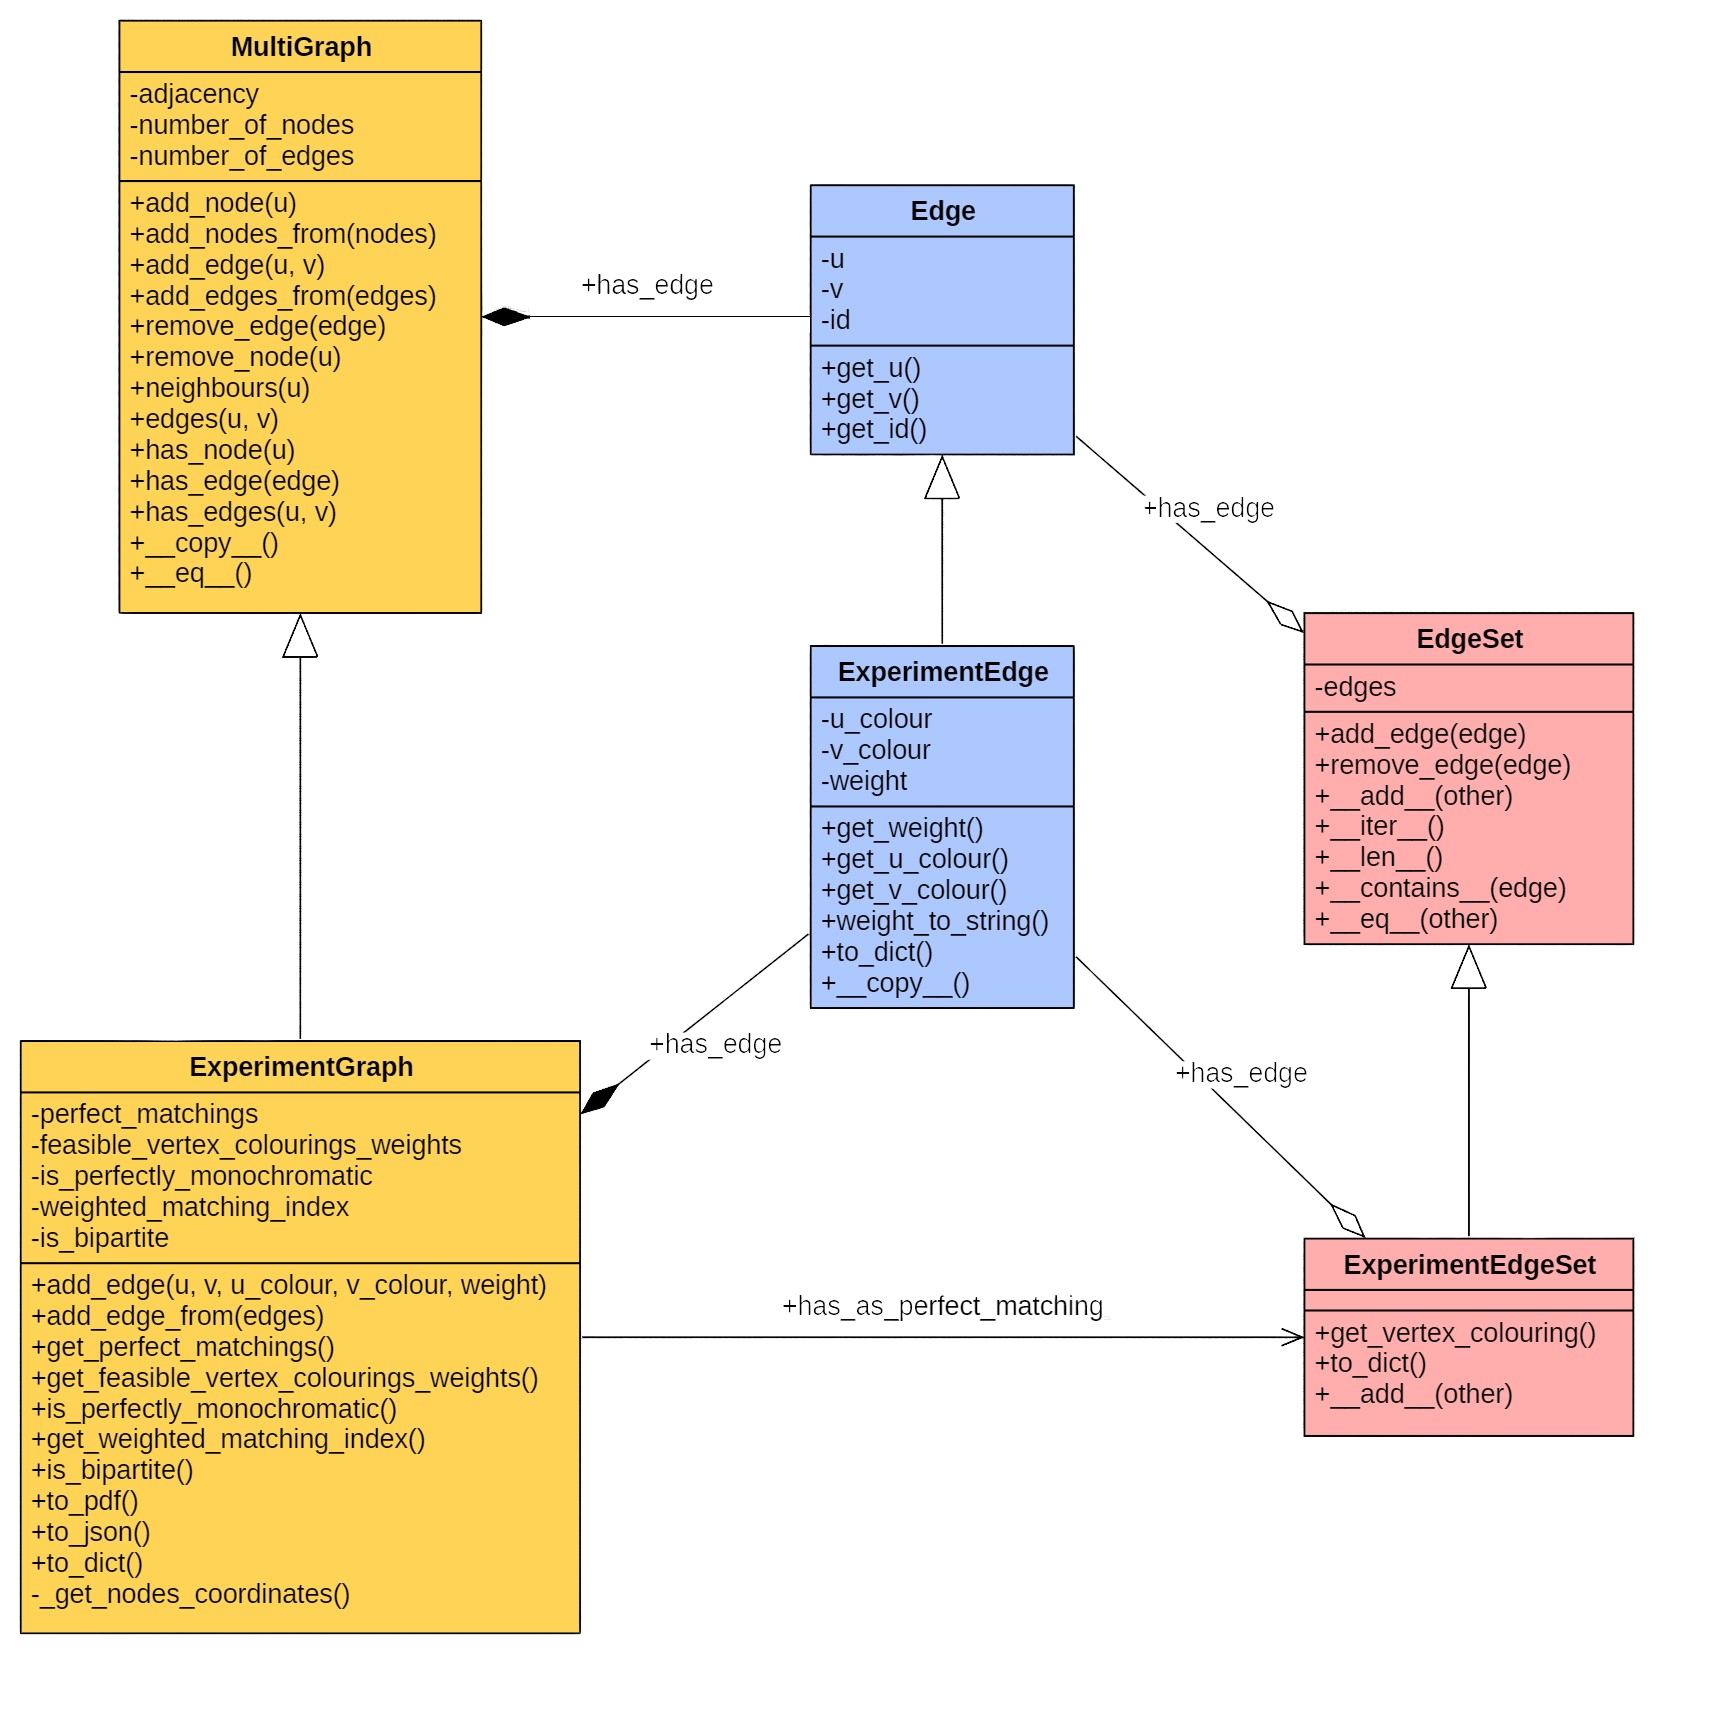
\includegraphics[scale=0.25]{figures/new_results/egpi/structure_diagram}
    \caption{Structure diagram of EGPI showing the important relations between the different implemented data structures. Most of the implemented methods of the program are shown in the diagram.}
    \label{fig:structure_diagram}
\end{figure}

Here is an exhaustive list of all non-trivial experiment graphs' properties we are interested to compute, and the algorithms we use in EGPI to do so.

\begin{enumerate}
    \item \textbf{Their perfect matchings:} to find all the perfect matchings of a graph, EGPI uses an algorithm written in pseudocode in algorithm~\ref{alg:perfect_matchings}.

        \begin{algorithm}
            \caption{Find all perfect matchings of an experiment graph $G$}
            \label{alg:perfect_matchings}
            \begin{algorithmic}
                \Require $G$ is an experiment graph
                \If{$G$ has no node}
                    \State The only perfect matching is $\varnothing$
                \ElsIf{$G$ has nodes}
                    \State $PMs$ $\gets$ empty list
                    \State choose a random node $u \in V(G)$
                    \ForAll{$v \in$ neighbours of $u$}
                        \State $subPMs \gets$ all perfect matchings of $G$ without $u$ and $v$
                        \ForAll{$subPM \in subPMs$}
                            \ForAll{$e \in$ edges between $u$ and $v$}
                                \State add $subPM \cup e$ to $PMs$
                            \EndFor
                        \EndFor
                    \EndFor
                \EndIf
                \State \Return PMs
            \end{algorithmic}
        \end{algorithm}

        \paragraph{Complexity of algorithm \ref {alg:perfect_matchings}:}
        The algorithm is a depth first search (DFS) algorithm.
        In the worst case scenario, $G_k^w$ is a complete graph with $n$ vertices.
        In other words, each node has $n-1$ neighbours in $G_k^w$.
        Also, at each recursive step of the algorithm, we remove $2$ nodes from the graph.
        This means that the depth of the search tree is $\frac{n}{2}$.
        The running time of this search algorithm is then $O\left(n^\frac{n}{2}\right)$. \\

    \item \textbf{The weights of their feasible vertex colourings:} according to their definition~\ref{def:feasible_vertex_colouring}, finding the feasible vertex colourings of an experiment graph requires to find their perfect matchings.
        The next steps to find them and their weights are simpler and are described in algorithm~\ref{alg:feasible_vertex_colourings}.

        \begin{algorithm}
            \caption{Find all feasible vertex colourings of an experiment graph $G_k^w$}
            \label{alg:feasible_vertex_colourings}
            \begin{algorithmic}
                \Require $G_k^w$ is an experiment graph
                \State $PMs \gets$ all perfect matchings of $G_k^w$
                \State $FVCs \gets$ empty Python dictionary
                \ForAll{$PM \in PMs$}
                    \State $FVC \gets$ feasible vertex colouring induced by $PM$
                    \State $w \gets$ weight of $PM$
                    \State $FVCs[FVC] \gets w$
                \EndFor
                \State \Return $FVCs$
            \end{algorithmic}
        \end{algorithm}

        The hardest step of this algorithm is to find all the perfect matchings of $G_k^w$.
        Therefore, the complexity of this algorithm is the same as the one of algorithm~\ref{alg:perfect_matchings}, which is $O\left(n^\frac{n}{2}\right)$ in the worst case.

    \item \textbf{If the graph is perfectly monochromatic:} by definition~\ref{def:perfectly_monochromatic_graph}, finding if an experiment graph is perfectly monochromatic or not just requires looking at all its feasible vertex colourings.
        This is done in algorithm~\ref{alg:perfectly_monochromatic}.

        \begin{algorithm}
            \caption{Check if an experiment graph $G_k^w$ is perfectly monochromatic}
            \label{alg:perfectly_monochromatic}
            \begin{algorithmic}
                \Require $G_k^w$ is an experiment graph
                \State $FVCs \gets$ all feasible vertex colourings of $G$
                \State $isPM \gets$ True
                \ForAll{$FVC \in FVCs$}
                    \If{FVC is monochromatic and $w(FVC) \neq 1$}
                        \State $isPM \gets$ False
                    \ElsIf{FVC is not monochromatic and $w(FVC) \neq 0$}
                        \State $isPM \gets$ False
                    \EndIf
                \EndFor
                \State \Return $isPM$
            \end{algorithmic}
        \end{algorithm}

        The only hard step of this algorithm is to find all the feasible vertex colourings of $G_k^w$.
        Therefore, the complexity of this algorithm is the same as the one of algorithm~\ref{alg:feasible_vertex_colourings}, which is $O\left(n^\frac{n}{2}\right)$ in the worst case.

    \item \textbf{The weighted matching index of the graph:} defined in definition~\ref{def:weighted_matching_index}, the weighted matching index of a perfectly monochromatic experiment graph is the number of monochromatic feasible vertex colourings in this graph.
        If the graph is not perfectly monochromatic, the weighted matching index is $0$ by definition.
        EGPI uses the algorithm~\ref{alg:weighted_matching_index} to compute the weighted matching index of a graph.
        \begin{algorithm}
            \caption{Compute the weighted matching index of an experiment graph $G_k^w$}
            \label{alg:weighted_matching_index}
            \begin{algorithmic}
                \Require $G_k^w$ is an experiment graph
                \State $FVCs \gets$ all feasible vertex colourings of $G_k^w$
                \State $isPM \gets$ is $G_k^w$ perfectly monochromatic ?
                \If{$isPM$}
                    \State $c \gets 0$
                    \ForAll{$FVC \in FVCs$}
                        \If{$w(FVC) = 1$}
                            \State $c \gets c + 1$
                        \EndIf
                    \EndFor
                    \State \Return $c$
                \Else
                    \State \Return $0$
                \EndIf
            \end{algorithmic}
        \end{algorithm}

        Again, the complexity of this algorithm is determined by the one of algorithm~\ref{alg:feasible_vertex_colourings}, which is $O\left(n^\frac{n}{2}\right)$ in the worst case.

    \item \textbf{If the graph is bipartite:} finding if a graph is bipartite or not is a well-known problem in graph theory.
        EGPI uses the following greedy algorithm to find if a graph is bipartite or not.
        The algorithm is written in algorithm~\ref{alg:bipartite}.
        \begin{algorithm}
            \caption{Check if an experiment graph $G_k^w$ is bipartite}
            \label{alg:bipartite}
            \begin{algorithmic}
                \Require $G_k^w$ is an experiment graph
                \State $Q \gets$ empty queue
                \State add $v_0 \in V(G_k^w)$ to $Q$
                \State colour of $v_0 \gets$ red
                \State $isBipartite \gets$ True
                \While{$Q$ is not empty}
                    \State $u \gets$ pop $Q$
                    \ForAll{$v \in$ neighbours of $u$}
                        \If{colour of $v$ is not defined}
                            \State colour of $v \gets$ opposite colour of $u$
                            \State add $v$ to $Q$
                        \ElsIf{colour of $v$ is the same as colour of $u$}
                            \State $isBipartite \gets$ False
                        \EndIf
                    \EndFor
                \EndWhile
                \State \Return $isBipartite$
            \end{algorithmic}
        \end{algorithm}

        This algorithm visits all the nodes of $G_k^w$ only once.
        Therefore, its complexity is $\mathcal{O}(n)$, where $n$ is the number of vertices of $G_k^w$.

\end{enumerate}


\section{Realized experiments with EGPI}
\label{sec:realized_experiments}

In this section, I present some of the experiments I realized with EGPI. The goal of these experiments was to find interesting properties of experiment graphs, and to try to find a counter-example to the Krenn's conjecture.\\

\subsection{Research for counter-examples}
\label{subsec:research-for-counter-examples}

The first experiment I realized with EGPI was to try to find a counter-example to the Krenn's conjecture.
To do so, I performed different random experiment graphs research processes, defined in definition~\ref{def:random_experiment_graphs_research_process}.
Each of these processes used the following parameters.

\begin{itemize}
    \item The number of trials was $m = 10^6$.
    \item The possible colours of the edges were $L_{colours} = \{red, green\}$.
    \item The possible complex weights of the edges were $L_{weights} = \{-1, 1, -i, i\}$.
\end{itemize}

I performed $21$ different random experiment graphs research processes, with $n \in {6, 8, 10}$ and $b \in \{1, 2, 3, 4, 5, 6\}$.

On all the $21$ millions generated candidate graphs, none of them was perfectly monochromatic.
This result is a new argument in favour of the Krenn's conjecture, at least for graphs that have less than $10$ vertices.
Nevertheless, it does not constitute a proof of it in any case, and I encourage future researchers to continue looking for counterexamples to it alongside their researches (by using EGPI or any other tool). \\


\subsection{Research for perfectly monochromatic graphs with a weighted matching index of $2$}
\label{subsec:research-for-graphs-with-c-of-2}

The second experiment I realized with EGPI was to try to find perfectly monochromatic graphs that have a weighted matching index of $2$.
These graphs are authorized by the Krenn's conjecture, and their properties are interesting to study.
Indeed, understanding better the structure of these graphs might help researchers to find new ideas in their seek for a proof to the conjecture.\\

But this is not the main and only interest of the experiment.
Exploring this class of experiment graphs is a great way to test the different functionalities of EGPI, and to experimentally check the impact of the different parameters of the program.
Using the following parameters,

\begin{itemize}
    \item The number of trials was $m = 10^6$.
    \item The possible colours of the edges were $L_{colours} = \{red, green\}$.
    \item The possible complex weights of the edges were $L_{weights} = \{-1, 1, -i, i\}$.
\end{itemize}

I performed $15$ different random experiment graphs research processes, with $n \in {6, 8, 10}$ and $b \in \{1, 2, 3, 4, 5\}$.
I got results summarized in figure~\ref{fig:results-experiment}.

\begin{figure}[H]
    \centering
    \begin{tabular}{ |p{1cm}||p{1.5cm}|p{1.5cm}|p{1.5cm}|p{1.5cm}|p{1.5cm}|p{1.5cm}|  }
        \hline
        \multicolumn{7}{|c|}{Results of the experiment} \\
        \hline
        $n$ & $b = 1$ & $b = 2$ & $b = 3$ & $b = 4$ & $b = 5$ & total \\
        \hline
        $6 $ & $103$ & $18$ & $4$ & $0$ & $0$ & $125$ \\
        $8 $ & $39$  & $1$  & $0$ & $0$ & $0$ & $40$  \\
        $10$ & $3$   & $0$  & $0$ & $0$ & $0$ & $3$   \\
        \hline
    \end{tabular}
    \caption{Results of $3$ different random experiment graphs research process with $n=6$, $n=8$ and $n=10$ respectively.}
    \label{fig:results-experiment}
\end{figure}

Here is an example of discovered perfectly monochromatic graph by the program.

\begin{figure}[H]
    \centering
    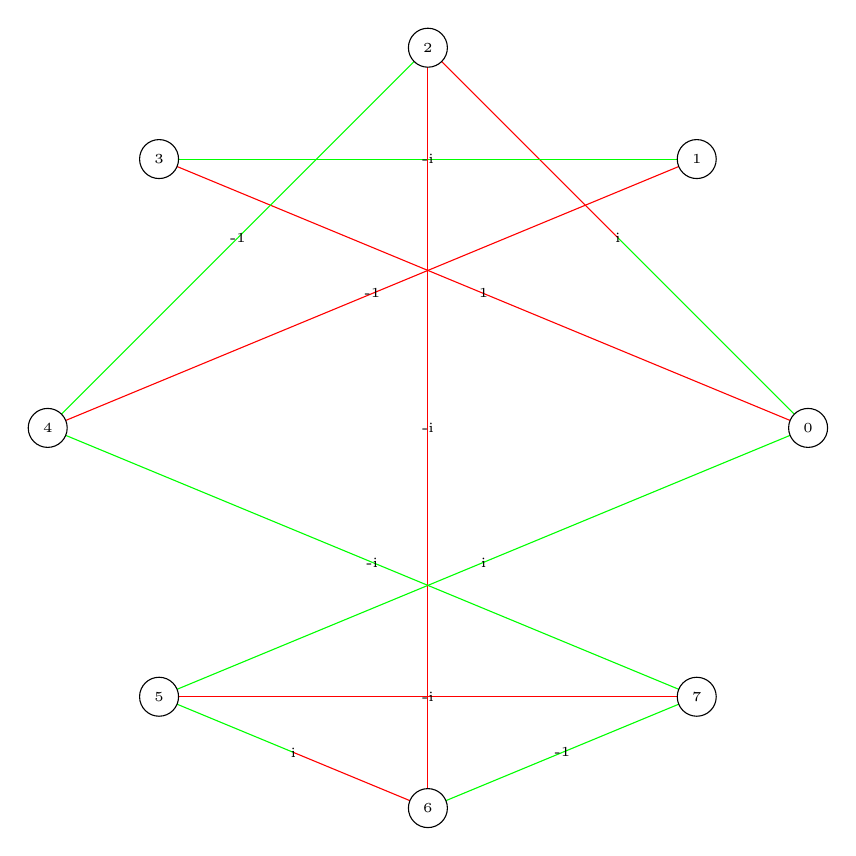
\begin{tikzpicture}
    \tikzstyle{every node}=[font=\tiny]
        \draw [style=thin, color=green] (4.82842712474619,0.0) to (2.414213562373095,2.414213562373095);
        \draw [style=thin, color=red] (2.414213562373095,2.414213562373095) to (2.9565589116183395e-16,4.82842712474619);
        \node [style=circle, draw=none] at (2.414213562373095,2.414213562373095) {i};
        \draw [style=thin, color=red] (4.82842712474619,0.0) to (0.7071067811865477,1.7071067811865475);
        \draw [style=thin, color=red] (0.7071067811865477,1.7071067811865475) to (-3.4142135623730945,3.414213562373095);
        \node [style=circle, draw=none] at (0.7071067811865477,1.7071067811865475) {1};
        \draw [style=thin, color=green] (4.82842712474619,0.0) to (0.707106781186547,-1.7071067811865472);
        \draw [style=thin, color=green] (0.707106781186547,-1.7071067811865472) to (-3.414213562373096,-3.4142135623730945);
        \node [style=circle, draw=none] at (0.707106781186547,-1.7071067811865472) {i};
        \draw [style=thin, color=green] (3.414213562373095,3.4142135623730945) to (2.220446049250313e-16,3.414213562373095);
        \draw [style=thin, color=green] (2.220446049250313e-16,3.414213562373095) to (-3.4142135623730945,3.414213562373095);
        \node [style=circle, draw=none] at (2.220446049250313e-16,3.414213562373095) {-i};
        \draw [style=thin, color=red] (3.414213562373095,3.4142135623730945) to (-0.7071067811865475,1.7071067811865475);
        \draw [style=thin, color=red] (-0.7071067811865475,1.7071067811865475) to (-4.82842712474619,5.913117823236679e-16);
        \node [style=circle, draw=none] at (-0.7071067811865475,1.7071067811865475) {-1};
        \draw [style=thin, color=green] (2.9565589116183395e-16,4.82842712474619) to (-2.414213562373095,2.4142135623730954);
        \draw [style=thin, color=green] (-2.414213562373095,2.4142135623730954) to (-4.82842712474619,5.913117823236679e-16);
        \node [style=circle, draw=none] at (-2.414213562373095,2.4142135623730954) {-1};
        \draw [style=thin, color=red] (2.9565589116183395e-16,4.82842712474619) to (-2.9565589116183395e-16,0.0);
        \draw [style=thin, color=red] (-2.9565589116183395e-16,0.0) to (-8.869676734855019e-16,-4.82842712474619);
        \node [style=circle, draw=none] at (-2.9565589116183395e-16,0.0) {-i};
        \draw [style=thin, color=green] (-4.82842712474619,5.913117823236679e-16) to (-0.7071067811865479,-1.7071067811865477);
        \draw [style=thin, color=green] (-0.7071067811865479,-1.7071067811865477) to (3.414213562373094,-3.414213562373096);
        \node [style=circle, draw=none] at (-0.7071067811865479,-1.7071067811865477) {-i};
        \draw [style=thin, color=green] (-3.414213562373096,-3.4142135623730945) to (-1.7071067811865483,-4.121320343559642);
        \draw [style=thin, color=red] (-1.7071067811865483,-4.121320343559642) to (-8.869676734855019e-16,-4.82842712474619);
        \node [style=circle, draw=none] at (-1.7071067811865483,-4.121320343559642) {i};
        \draw [style=thin, color=red] (-3.414213562373096,-3.4142135623730945) to (-8.881784197001252e-16,-3.414213562373095);
        \draw [style=thin, color=red] (-8.881784197001252e-16,-3.414213562373095) to (3.414213562373094,-3.414213562373096);
        \node [style=circle, draw=none] at (-8.881784197001252e-16,-3.414213562373095) {-i};
        \draw [style=thin, color=green] (-8.869676734855019e-16,-4.82842712474619) to (1.7071067811865466,-4.121320343559643);
        \draw [style=thin, color=green] (1.7071067811865466,-4.121320343559643) to (3.414213562373094,-3.414213562373096);
        \node [style=circle, draw=none] at (1.7071067811865466,-4.121320343559643) {-1};
        \node [style=circle, fill=white, draw=black] (0) at (4.82842712474619,0.0) {0};
        \node [style=circle, fill=white, draw=black] (1) at (3.414213562373095,3.4142135623730945) {1};
        \node [style=circle, fill=white, draw=black] (2) at (2.9565589116183395e-16,4.82842712474619) {2};
        \node [style=circle, fill=white, draw=black] (3) at (-3.4142135623730945,3.414213562373095) {3};
        \node [style=circle, fill=white, draw=black] (4) at (-4.82842712474619,5.913117823236679e-16) {4};
        \node [style=circle, fill=white, draw=black] (5) at (-3.414213562373096,-3.4142135623730945) {5};
        \node [style=circle, fill=white, draw=black] (6) at (-8.869676734855019e-16,-4.82842712474619) {6};
        \node [style=circle, fill=white, draw=black] (7) at (3.414213562373094,-3.414213562373096) {7};
    \end{tikzpicture}
    \caption{A perfectly monochromatic graph of size $8$ vertices, with a weighted matching index of $2$, discovered by EGPI during the experiment.}
    \label{fig:egpi_graph_example}
\end{figure}

From the results in figure~\ref{fig:results-experiment}, we can do the following observations.
Firstly, it is a lot harder to find perfectly monochromatic graphs in these conditions when their size is bigger.
Indeed, the number of possibilities grows exponentially with the number of vertices, and the probability to find a perfectly monochromatic graph decreases.
Secondly, the complexity bound has a big impact on the number of found graphs: a higher complexity bound results in a smaller number of found graphs.
This was expected, since the graphs generated with a higher complexity bound have higher chances to have more edges and perfect matchings.
The probability that all these randomly generated edges and perfect matchings together satisfy the definition~\ref{def:perfectly_monochromatic_graph} are small.\\

The last thing I am interested in is to count bipartite graphs among all the perfectly monochromatic graphs found.
The result is the following: \textbf{none} of the perfectly monochromatic graphs found were bipartite.
This is an alluring new observation: indeed, it is consistent with the arguments we used in the proofs of lemmas~\ref{lem:one_neg_edge} and~\ref{lem:2_positive_colour_classes_forbidden}.
One of the observations these proofs used is that, in these particular cases, the perfectly monochromatic graphs found were not bipartite.
This allows me to formulate the following conjecture.

\begin{conjecture}
    \label{con:bipartite_perfectly_monochromatic}
    Let $G_k^w$ be a non-redundant perfectly monochromatic graph that respects the following properties.
    \begin{itemize}
        \item $\Tilde{c}(G, k, w) \geq 2$
        \item $\forall e \in E(G_k^w), w(e) \in \{-1, 1, -i, i\}$
        \item $G_k^w$ has at least one non-monochromatic feasible vertex colouring.
    \end{itemize}
    Then, $G_k^w$ is not bipartite.
\end{conjecture}

This conjecture might constitute a new interesting subcase of the Krenn's conjecture to investigate in the future.


\section{Possible improvements for EGPI}
\label{sec:possible-improvements-for-egpi}

EGPI is a tool that can still be improved in many ways.\\

Firstly, currently it does not offer the functionality of generating only non-isomorphic graphs.
This functionality could be interesting if the user wants to count the number of different graphs generated by the tool.
This could be coded from scratch, or by using an external program.
For instance, in Python, the package \textit{NetworkX} offers a function to check if $2$ graphs are isomorphic or not~\cite{networkx}.
A more common program used a lot in the field of graph theory is Nauty, a program originally designed by Brendan McKay~\cite{MCKAY201494}.
Using it would offer a lot of advantages, but it would require to write a wrapper around it to use it in Python.
Indeed, Nauty is written in C. \\

A second improvement that could be brought to EGPI is to improve the efficiency of the algorithms used to find the perfect matchings of a graph.
Indeed, this step bounds the efficiency of most of the tasks performed by EGPI\@.
Improving this algorithm would allow the program to search more graphs in a given time, and to find more results in general.
One idea to improve it could be to look at the Edmonds' Blossom algorithm, an algorithm to find a single perfect matching in a graph~\cite{Edmonds_1965}.
It has to be determined whether this algorithm can be adapted to find all perfect matchings of a graph.\\

\setcounter{secnumdepth}{-1}

\chapter{Conclusion}
\label{ch:conclusion}

In this master thesis, we started by understanding and summarizing the concept of the Krenn's conjecture: a conjecture about perfect matchings and their intersections in edge-weighted edge-bi-coloured multigraphs.\cite{wordpress}
We dived deeper in the connection between this conjecture and quantum physics, investigated for the first time by Mario Krenn in~\cite{Krenn_2017}.
Mario Krenn indeed discovered that the (non-)existence of certain specific graphs could lead to the (non-)feasibility to create specific quantum states, called $GHZ$-states, through the use of certain experiments.
Being able to create such states is a key point in quantum computing~\cite{gu2020compact} and cryptography~\cite{pivoluska2018layered}.
This discovery was the starting point of his conjecture in graph theory, which remains unsolved.\\

We then focused on dressing a state of the art of the research on the Krenn's conjecture.
In it, we could see that the conjecture was already solved for real, positive weights by Bogdanov in~\cite{bogdanov}.
We also spoke about Chandran and Gajjala, who proved the conjecture in the special case of graphs that have a matching index (defined in~\ref{def:matching_index}) different from 1~\cite{chandran}.
In that same paper, they could find some upper bounds on the weighted matching index in terms of minimum degree and of edge connectivity.
Their researches were extremely valuable for us, as they introduced a lot of notations and concepts that we used in our own work.\\

After that, we adopted a theoretical approach to find new interesting results related to the problem.
We first tried to perform problem reductions to find out what restrained cases were interesting to study.
By doing so, we discovered that the study of non-redundant experiment graphs (defined in~\ref{def:redundant-experiment-graph}) with integer weights could be reduced to the study of redundant experiment graphs that have weights included in $\{-1, 1\}$.
We then focused on proving some new special cases of the Krenn's conjecture.
Our main results are the following: we could extend Bogdanov's results\cite{bogdanov} by allowing one weight to be negative in the absence of bicoloured edges.
This attempt was a success, and encouraged us to extend the used arguments to a more general case.
This is how we came by with what I consider to be the main result of this master thesis, formulated in Lemma~\ref{lem:2_positive_colour_classes_forbidden}.

\paragraph{Lemma~\ref{lem:2_positive_colour_classes_forbidden}}
Let $G_\mu^w$ be a simple perfectly monochromatic graph that has only real weights, and that has at least $2$ colour classes that have only positive weighted edges.
Then, if $G$ is not isomorphic to $K_4$, $\Tilde{c}(G, \mu, w) \leq 2$.\\


At last, we adopted a more experimental approach to the problem by looking for counter-examples to the Krenn's conjecture.
In practice, this was done through the implementation of a new program called EGPI (Experiment Graphs Properties Identifier) — a program that generates random experiment graphs and checks properties related to the Krenn's conjecture on them.
In my opinion, such a tool was currently missing in the researchers' community.
Indeed, finding interesting graphs to analyse or showcase by hand is hard, and the EGPI program could help in this task.
Also, even though I strongly believe the conjecture to be true at this point, it is not excluded that the EGPI program (or any similar tool) finds a counter-examples to it by chance one day.
Using EGPI, I looked for such counter-examples and could not find any, which reinforces my belief in the conjecture's truth.
EGPI also allowed me to analyse a big number of random perfectly monochromatic graphs with a weighted matching index of $2$, and to discover that none of them were bipartite.
Therefore, I finished my work by stating conjecture~\ref{con:bipartite_perfectly_monochromatic} about the non-existence of bipartite perfectly-monochromatic graphs in certain conditions.\\


\printglossary

\printglossary[type=\acronymtype]

\listoftheorems

%Bibliography
\nocite{*}
\printbibliography % [type=article,title=Articles]
% \printbibliography[type=misc,title=Other references]

\end{document}
